\documentclass[conference,10pt]{IEEEtran}

\usepackage[utf8]{inputenc}
\usepackage[T1]{fontenc}
\usepackage{amsmath,amssymb}
\usepackage{graphicx}
\usepackage{booktabs}
\usepackage{array}
\usepackage{url}
\usepackage{cite}
\usepackage[hidelinks]{hyperref}

\graphicspath{{figures/}}

\title{Statistical Analysis of Customer Spending and Ordering Behavior at Starbucks}

\author{
\IEEEauthorblockN{Naman Sudan, Priya Venugopal Nair, Sanjana Vivek Phalke, Varuna Vyomessh}
\IEEEauthorblockA{Department of Applied Data Intelligence\\
San Jose State University\\
DATA 202, Spring 2026}
}

\begin{document}
\maketitle

\begin{abstract}
We analyze 100{,}000 Starbucks customer orders to quantify what drives the per\nobreakdash-order spend and to test segment\nobreakdash-level differences using the mathematical and statistical methods taught in DATA 202. The analysis combines descriptive statistics, Pearson correlation, Chebyshev's inequality, distribution diagnostics, confidence intervals, two\nobreakdash-sample and paired $t$\nobreakdash-tests, two\nobreakdash-proportion $z$\nobreakdash-tests, empirical and Bayesian probability, a discrete random variable analysis of cart size, and a least\nobreakdash-squares linear model solved through the normal equations and verified by gradient descent. Cart size is the dominant order\nobreakdash-level driver of total spend with $r{\approx}0.90$. Mobile App orders spend on average \$5.58 more than non\nobreakdash-mobile orders, and after controlling for cart size and customizations the Mobile premium is still \$2.33. Rewards membership shifts spend up by a smaller \$1.63. The fitted linear model achieves $R^2{\approx}0.95$ on the training sample. We discuss how the same analysis pipeline could be deployed inside a Starbucks marketing or revenue\nobreakdash-management workflow.
\end{abstract}

\section{Introduction}

Starbucks operates one of the largest retail coffee networks in the world. Understanding what drives per\nobreakdash-order revenue at a single transaction is central to merchandising, mobile\nobreakdash-channel investment, and rewards\nobreakdash-program design. The DATA 202 syllabus covers measurements and sampling, descriptive statistics, correlation and covariance, distribution theorems, confidence intervals, hypothesis testing, probability and random variables, distributions, calculus and optimization, and linear algebra \cite{course202}. This report uses each of those tools on a single open dataset to answer one practical question: \emph{do customers spend more in certain channels or segments, and what variables actually move the per\nobreakdash-order spend?}

The contribution is methodological rather than novel. We treat the analysis as a complete worked example of the course content applied to a 100{,}000\nobreakdash-row real\nobreakdash-world dataset, with every formula written out, computed, and visualized. Sections are organized so that each block of analysis maps directly to one or two course lectures.

\section{Data Description}

\subsection{Source}
The dataset is the public \emph{Starbucks Customer Ordering Patterns} table on Kaggle \cite{kaggle}. Each row is a single customer order. The file contains 100{,}000 orders placed by 14{,}988 unique customers across 500 stores, with no missing values, between 2024\nobreakdash-01\nobreakdash-01 and 2025\nobreakdash-12\nobreakdash-30. There are 20 columns covering customer attributes, store attributes, channel, time, cart size, customizations, total spend, fulfillment time, drink category, food attachment, order\nobreakdash-ahead flag, and customer satisfaction.

\subsection{Variables}
The 20 columns split into qualitative and quantitative variables. Qualitative columns include \texttt{customer\_id}, \texttt{order\_id}, \texttt{order\_channel}, \texttt{store\_location\_type}, \texttt{region}, \texttt{customer\_age\_group}, \texttt{customer\_gender}, \texttt{drink\_category}, and three booleans (\texttt{is\_rewards\_member}, \texttt{has\_food\_item}, \texttt{order\_ahead}). Quantitative columns are \texttt{cart\_size}, \texttt{num\_customizations}, \texttt{total\_spend}, \texttt{fulfillment\_time\_min}, and \texttt{customer\_satisfaction} (treated as ordinal). The response variable in this study is \texttt{total\_spend}.

\subsection{Descriptive Statistics}
For the five quantitative columns we compute the mean, median, mode, standard deviation, variance, and the five\nobreakdash-number summary. Table~\ref{tab:desc} reports the values that drive the rest of the report. The mean and median of \texttt{total\_spend} are close (\$14.87 vs \$14.17) and the standard deviation is \$5.51, which is consistent with a roughly symmetric distribution with a slight right skew. The IQR fences flag only 1.42\% of orders as outliers on \texttt{total\_spend}; we keep them.

\begin{table}[!t]
\caption{Descriptive Statistics for Quantitative Variables}
\label{tab:desc}
\centering
\renewcommand{\arraystretch}{1.1}
\begin{tabular}{lrrrr}
\toprule
Variable & Mean & Median & SD & IQR \\
\midrule
total\_spend (\$)        & 14.87 & 14.17 & 5.51 & 7.34 \\
cart\_size               & 3.74  & 4.00  & 1.70 & 2.00 \\
num\_customizations      & 1.81  & 2.00  & 1.46 & 2.00 \\
fulfillment\_time\_min   & 4.55  & 4.40  & 1.55 & 2.10 \\
customer\_satisfaction   & 3.69  & 4.00  & 1.18 & 2.00 \\
\bottomrule
\end{tabular}
\end{table}

\subsection{Channel and Segment Mix}
About 42.5\% of orders are placed through the Mobile App, 28.0\% Drive\nobreakdash-Thru, 22.1\% In\nobreakdash-Store Cashier, and 7.4\% Kiosk. Rewards members account for 47.7\% of orders. Region, store location type, and drink category are roughly evenly distributed. The largest single segmentation effect on mean spend comes from the order channel: Mobile App orders average \$18.08 while the other three channels are tightly clustered near \$12.50.

\section{Mathematical and Statistical Methods}

This section states the formulas used in the rest of the paper. Each formula is taken directly from a DATA 202 lecture.

\subsection{Pearson Correlation and Sample Covariance}
For paired observations $(x_i, y_i)_{i=1}^{n}$, sample covariance and Pearson correlation are
\begin{equation}
\mathrm{Cov}(X,Y) = \frac{1}{n-1}\sum_{i=1}^{n}(x_i-\bar{x})(y_i-\bar{y}),
\label{eq:cov}
\end{equation}
\begin{equation}
r_{XY} = \frac{\mathrm{Cov}(X,Y)}{\sigma_X\,\sigma_Y}.
\label{eq:pearson}
\end{equation}

\subsection{Chebyshev's Inequality and the Empirical Rule}
Chebyshev's inequality holds for any distribution with finite mean and variance:
\begin{equation}
P(|X-\mu| < k\sigma) \;\ge\; 1 - \frac{1}{k^2}.
\label{eq:chebyshev}
\end{equation}
The empirical (68/95/99.7) rule is a tighter approximation that requires $X$ to be close to normal.

\subsection{Confidence Interval for a Mean}
The two\nobreakdash-sided $100(1-\alpha)\%$ confidence interval for $\mu$ from a sample of size $n$ is
\begin{equation}
\bar{x} \;\pm\; t_{\alpha/2,\,n-1}\,\frac{s}{\sqrt{n}}.
\label{eq:ci}
\end{equation}
For the sample sizes in this study ($n>10{,}000$) the $t$\nobreakdash-quantile is indistinguishable from $z=1.96$ at $\alpha=0.05$.

\subsection{Welch's Two-Sample $t$-test}
For two independent samples with sizes $n_1, n_2$, sample means $\bar{x}_1, \bar{x}_2$, and variances $s_1^2, s_2^2$, the Welch statistic is
\begin{equation}
t = \frac{\bar{x}_1 - \bar{x}_2}{\sqrt{\dfrac{s_1^2}{n_1}+\dfrac{s_2^2}{n_2}}}.
\label{eq:welch}
\end{equation}

\subsection{Paired $t$-test}
For matched pairs with within\nobreakdash-pair difference $d_i$, the test statistic is
\begin{equation}
t = \frac{\bar{d}}{s_d/\sqrt{n}}, \qquad H_0:\mu_d = 0.
\label{eq:paired}
\end{equation}

\subsection{Two-Proportion $z$-test}
\begin{equation}
z = \frac{\hat{p}_1 - \hat{p}_2}{\sqrt{\hat{p}(1-\hat{p})\!\left(\frac{1}{n_1}+\frac{1}{n_2}\right)}}, \quad \hat{p}=\frac{x_1+x_2}{n_1+n_2}.
\label{eq:zprop}
\end{equation}

\subsection{Empirical Probability, Conditional Probability, Bayes}
\begin{equation}
\hat{P}(A) = \frac{\#\{i:\,x_i \in A\}}{n}, \qquad
P(A\mid B) = \frac{P(A\cap B)}{P(B)},
\label{eq:emp}
\end{equation}
\begin{equation}
P(A\mid B) = \frac{P(B\mid A)\,P(A)}{P(B\mid A)\,P(A) + P(B\mid A^c)\,P(A^c)}.
\label{eq:bayes}
\end{equation}

\subsection{Discrete Random Variable Moments}
\begin{equation}
E[X] = \sum_k k\,\hat{p}(k), \quad
\mathrm{Var}(X) = \sum_k (k-E[X])^2\,\hat{p}(k).
\label{eq:rv}
\end{equation}

\subsection{Least Squares: Normal Equations and Gradient Descent}
With $y\in\mathbb{R}^n$, design matrix $X\in\mathbb{R}^{n\times p}$, and squared\nobreakdash-error loss
$J(\beta)=\|y-X\beta\|^2$, setting $\nabla_\beta J=0$ gives the normal equations
\begin{equation}
X^{\top}X\,\beta = X^{\top}y,\qquad \hat{\beta}=(X^{\top}X)^{-1}X^{\top}y.
\label{eq:normal}
\end{equation}
The same minimizer can be reached iteratively from
\begin{equation}
\beta_{t+1} = \beta_t - \eta\,\nabla_\beta J(\beta_t),
\quad \nabla_\beta J(\beta) = -2 X^{\top}(y-X\beta).
\label{eq:gd}
\end{equation}

\section{Analysis and Results}

\subsection{Order-Level Correlation and Covariance}
We compute (\ref{eq:cov}) and (\ref{eq:pearson}) on the order\nobreakdash-level numerical block. Cart size is the dominant driver of \texttt{total\_spend} with $r=0.900$, followed by \texttt{num\_customizations} ($r=0.409$). Fulfillment time and customer satisfaction are essentially uncorrelated with spend ($|r|<0.07$). Manual computation reproduces the pandas value to four decimal places: $\mathrm{Cov}(\texttt{cart\_size},\texttt{total\_spend})=8.4159$ and $r=0.9001$. Figure~\ref{fig:corr} shows the order\nobreakdash-level correlation heatmap and Figure~\ref{fig:scatter} shows the two predictor scatter plots that drive the model in Section~\ref{sec:linmodel}.

\begin{figure}[!t]
\centering
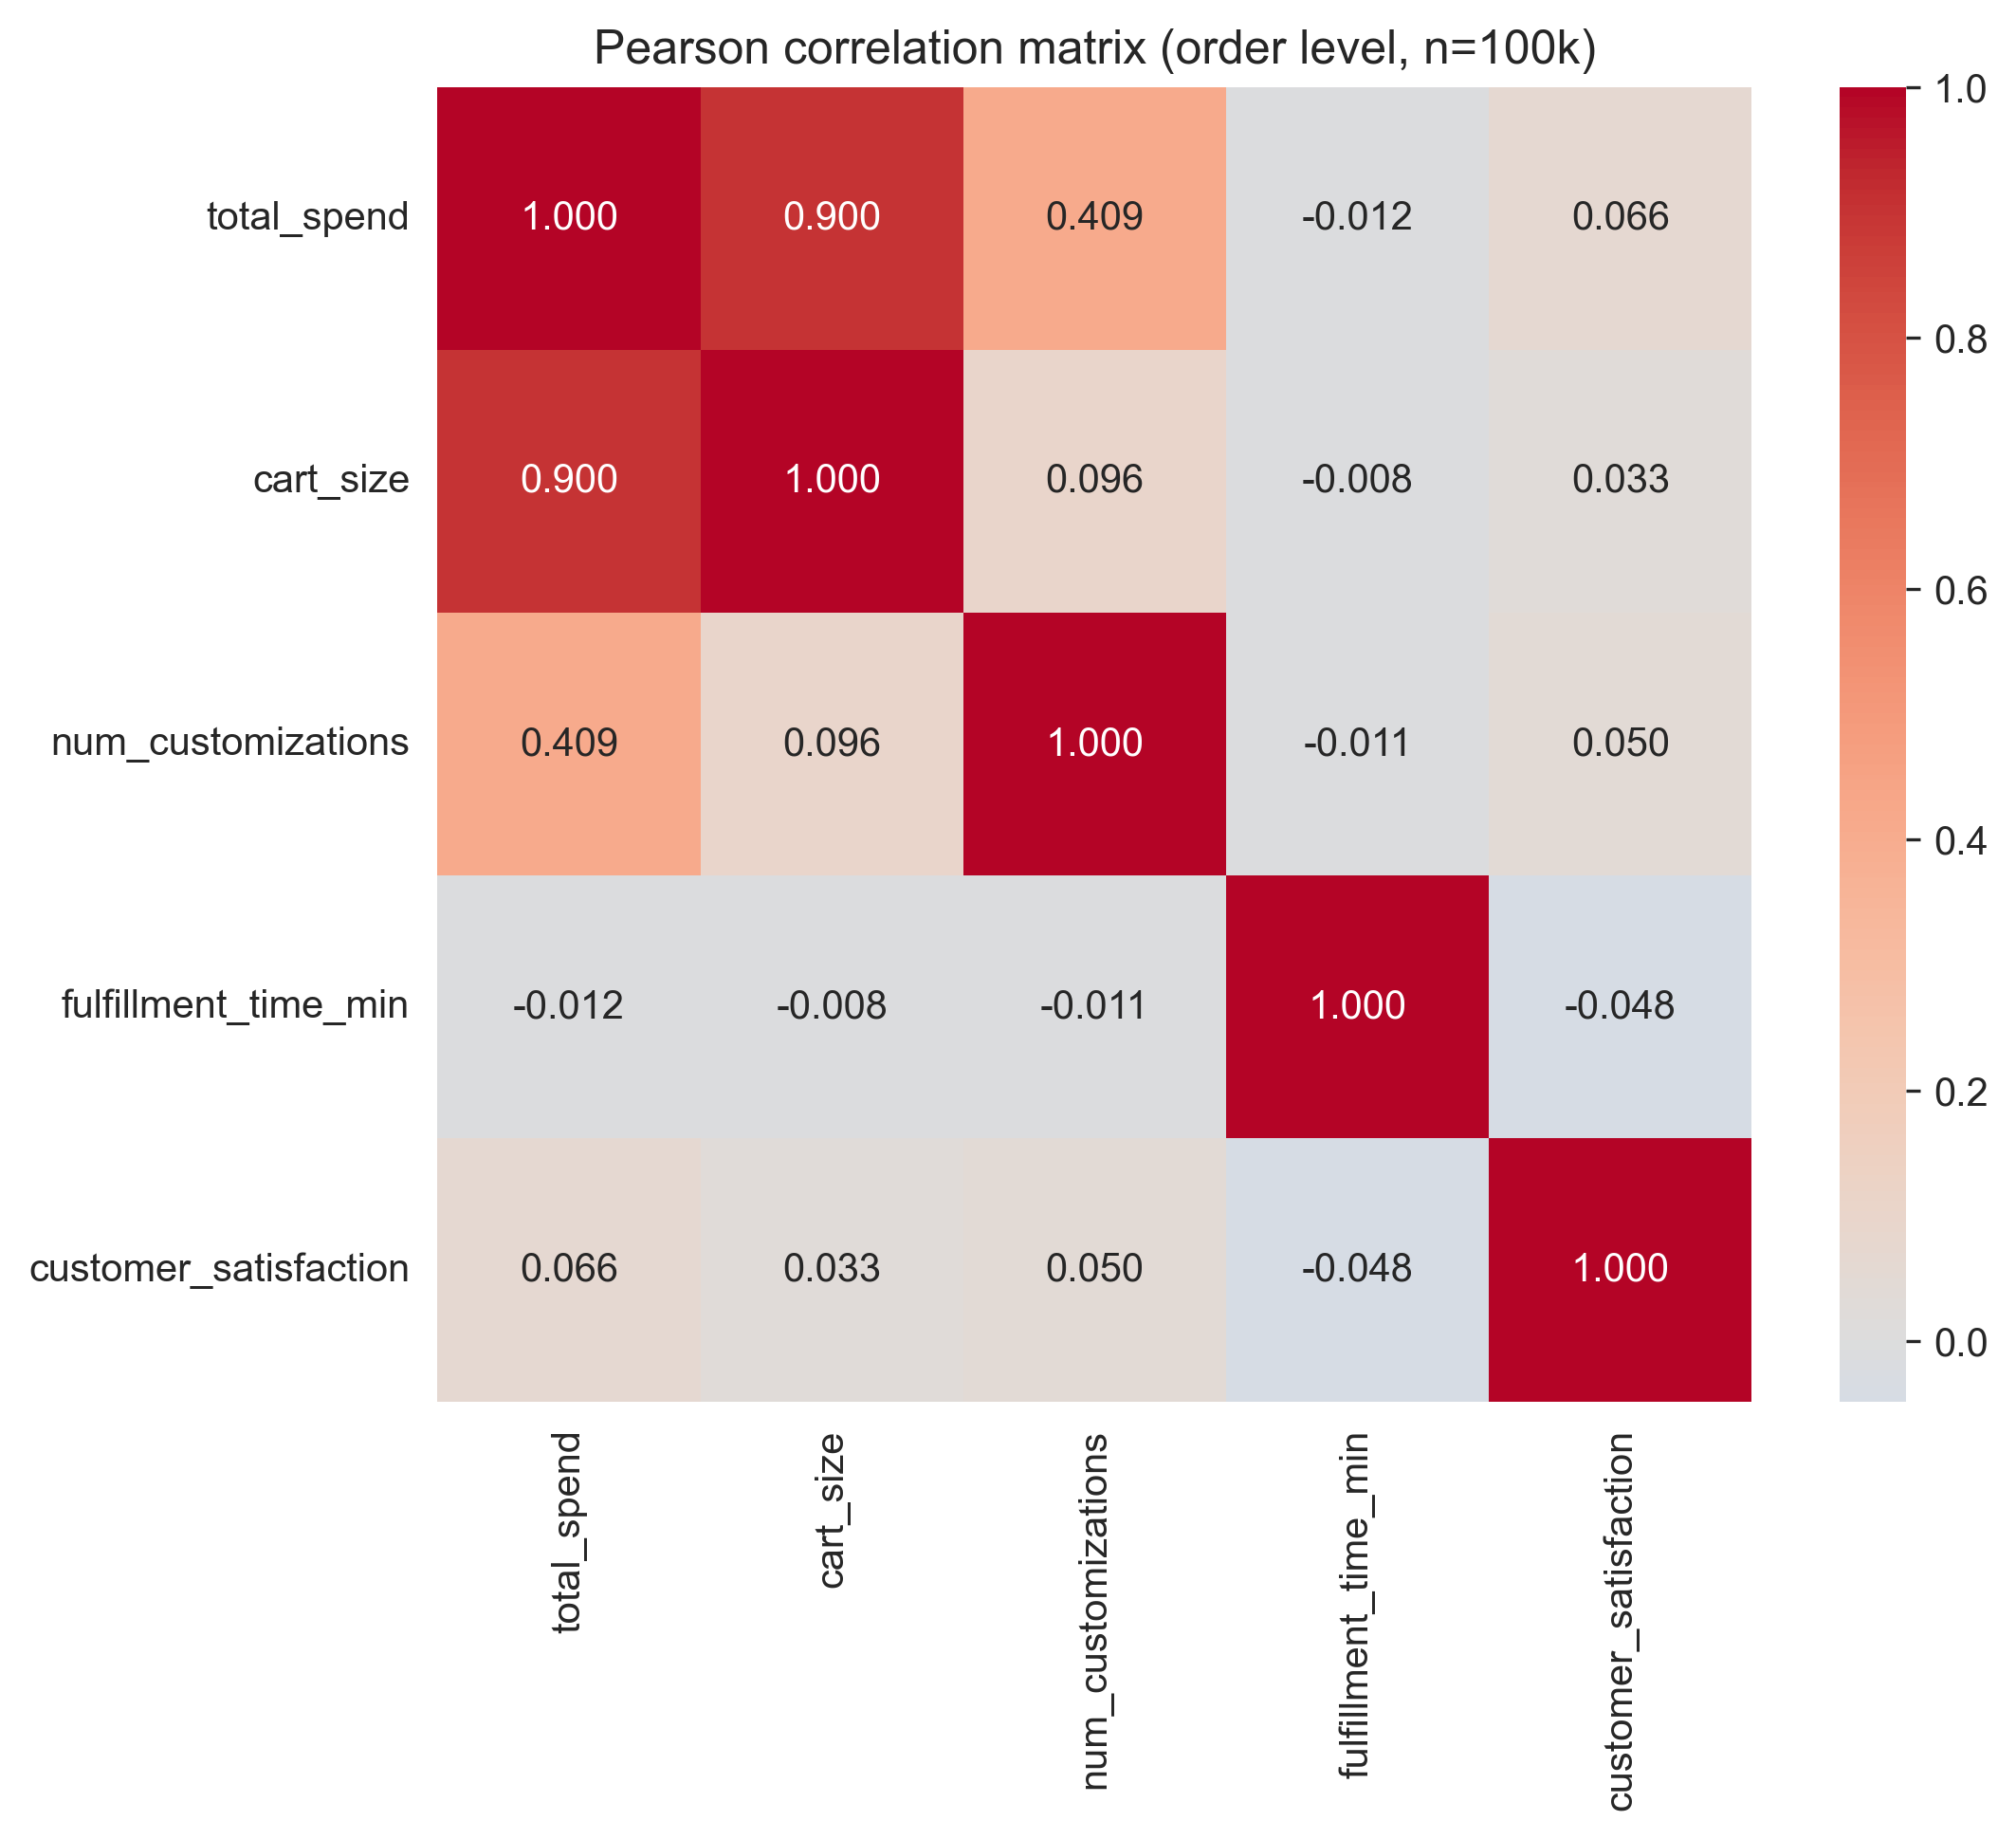
\includegraphics[width=0.95\columnwidth]{02_corr_heatmap_order_level.png}
\caption{Pearson correlation matrix at the order level ($n=100{,}000$).}
\label{fig:corr}
\end{figure}

\begin{figure}[!t]
\centering
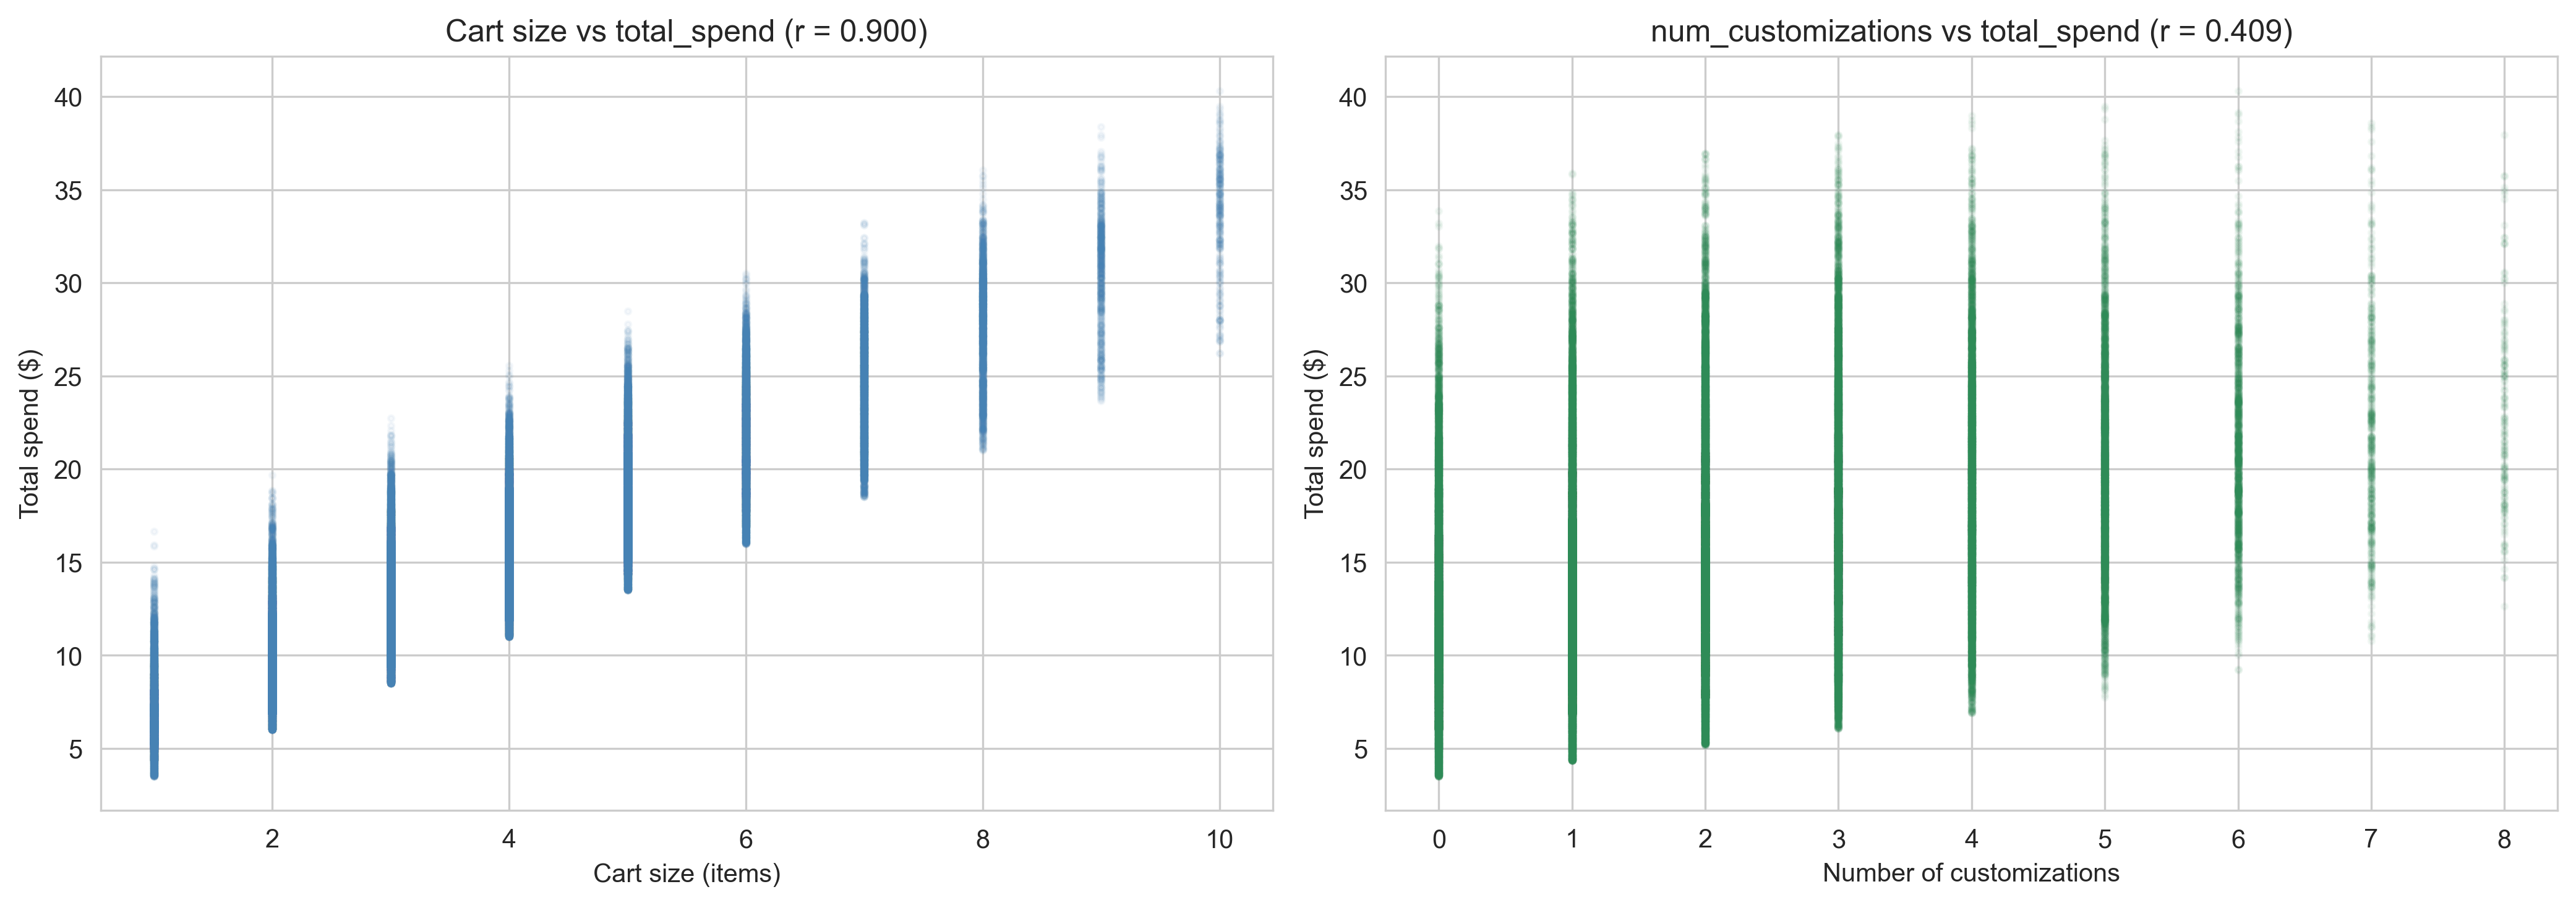
\includegraphics[width=\columnwidth]{02_scatter_predictors_vs_spend.png}
\caption{Order-level scatter plots of cart\_size and num\_customizations against total\_spend.}
\label{fig:scatter}
\end{figure}

A customer\nobreakdash-level aggregation was also computed for documentation but not used as the headline. Summing customizations within a customer inflates correlation with summed spend (from $r{=}0.41$ at the order level to $r{=}0.81$ at the customer level), and averaging cart size deflates it ($r{=}0.90$ to $r{=}0.30$). Both effects are sum\nobreakdash-of\nobreakdash-sums or averaging artifacts. The order\nobreakdash-level numbers are the right ones to interpret.

\subsection{Distribution of Total Spend}
Applying (\ref{eq:chebyshev}) to \texttt{total\_spend} with $\mu=14.87$ and $\sigma=5.51$ yields the bounds in Table~\ref{tab:cheb}. The actual within\nobreakdash-band shares are far above Chebyshev's worst case and very close to the empirical\nobreakdash-rule values, indicating that the distribution is much closer to normal than the worst case. Figure~\ref{fig:cheb} overlays the $\pm 2\sigma$ and $\pm 3\sigma$ bands on the histogram.

\begin{table}[!t]
\caption{Chebyshev vs Empirical Rule vs Actual for \texttt{total\_spend}}
\label{tab:cheb}
\centering
\renewcommand{\arraystretch}{1.1}
\begin{tabular}{cccc}
\toprule
$k$ & Chebyshev min. & Empirical rule & Actual \\
\midrule
2 & 75.00\% & 95.4\% & 95.83\% \\
3 & 88.89\% & 99.7\% & 99.34\% \\
\bottomrule
\end{tabular}
\end{table}

\begin{figure}[!t]
\centering
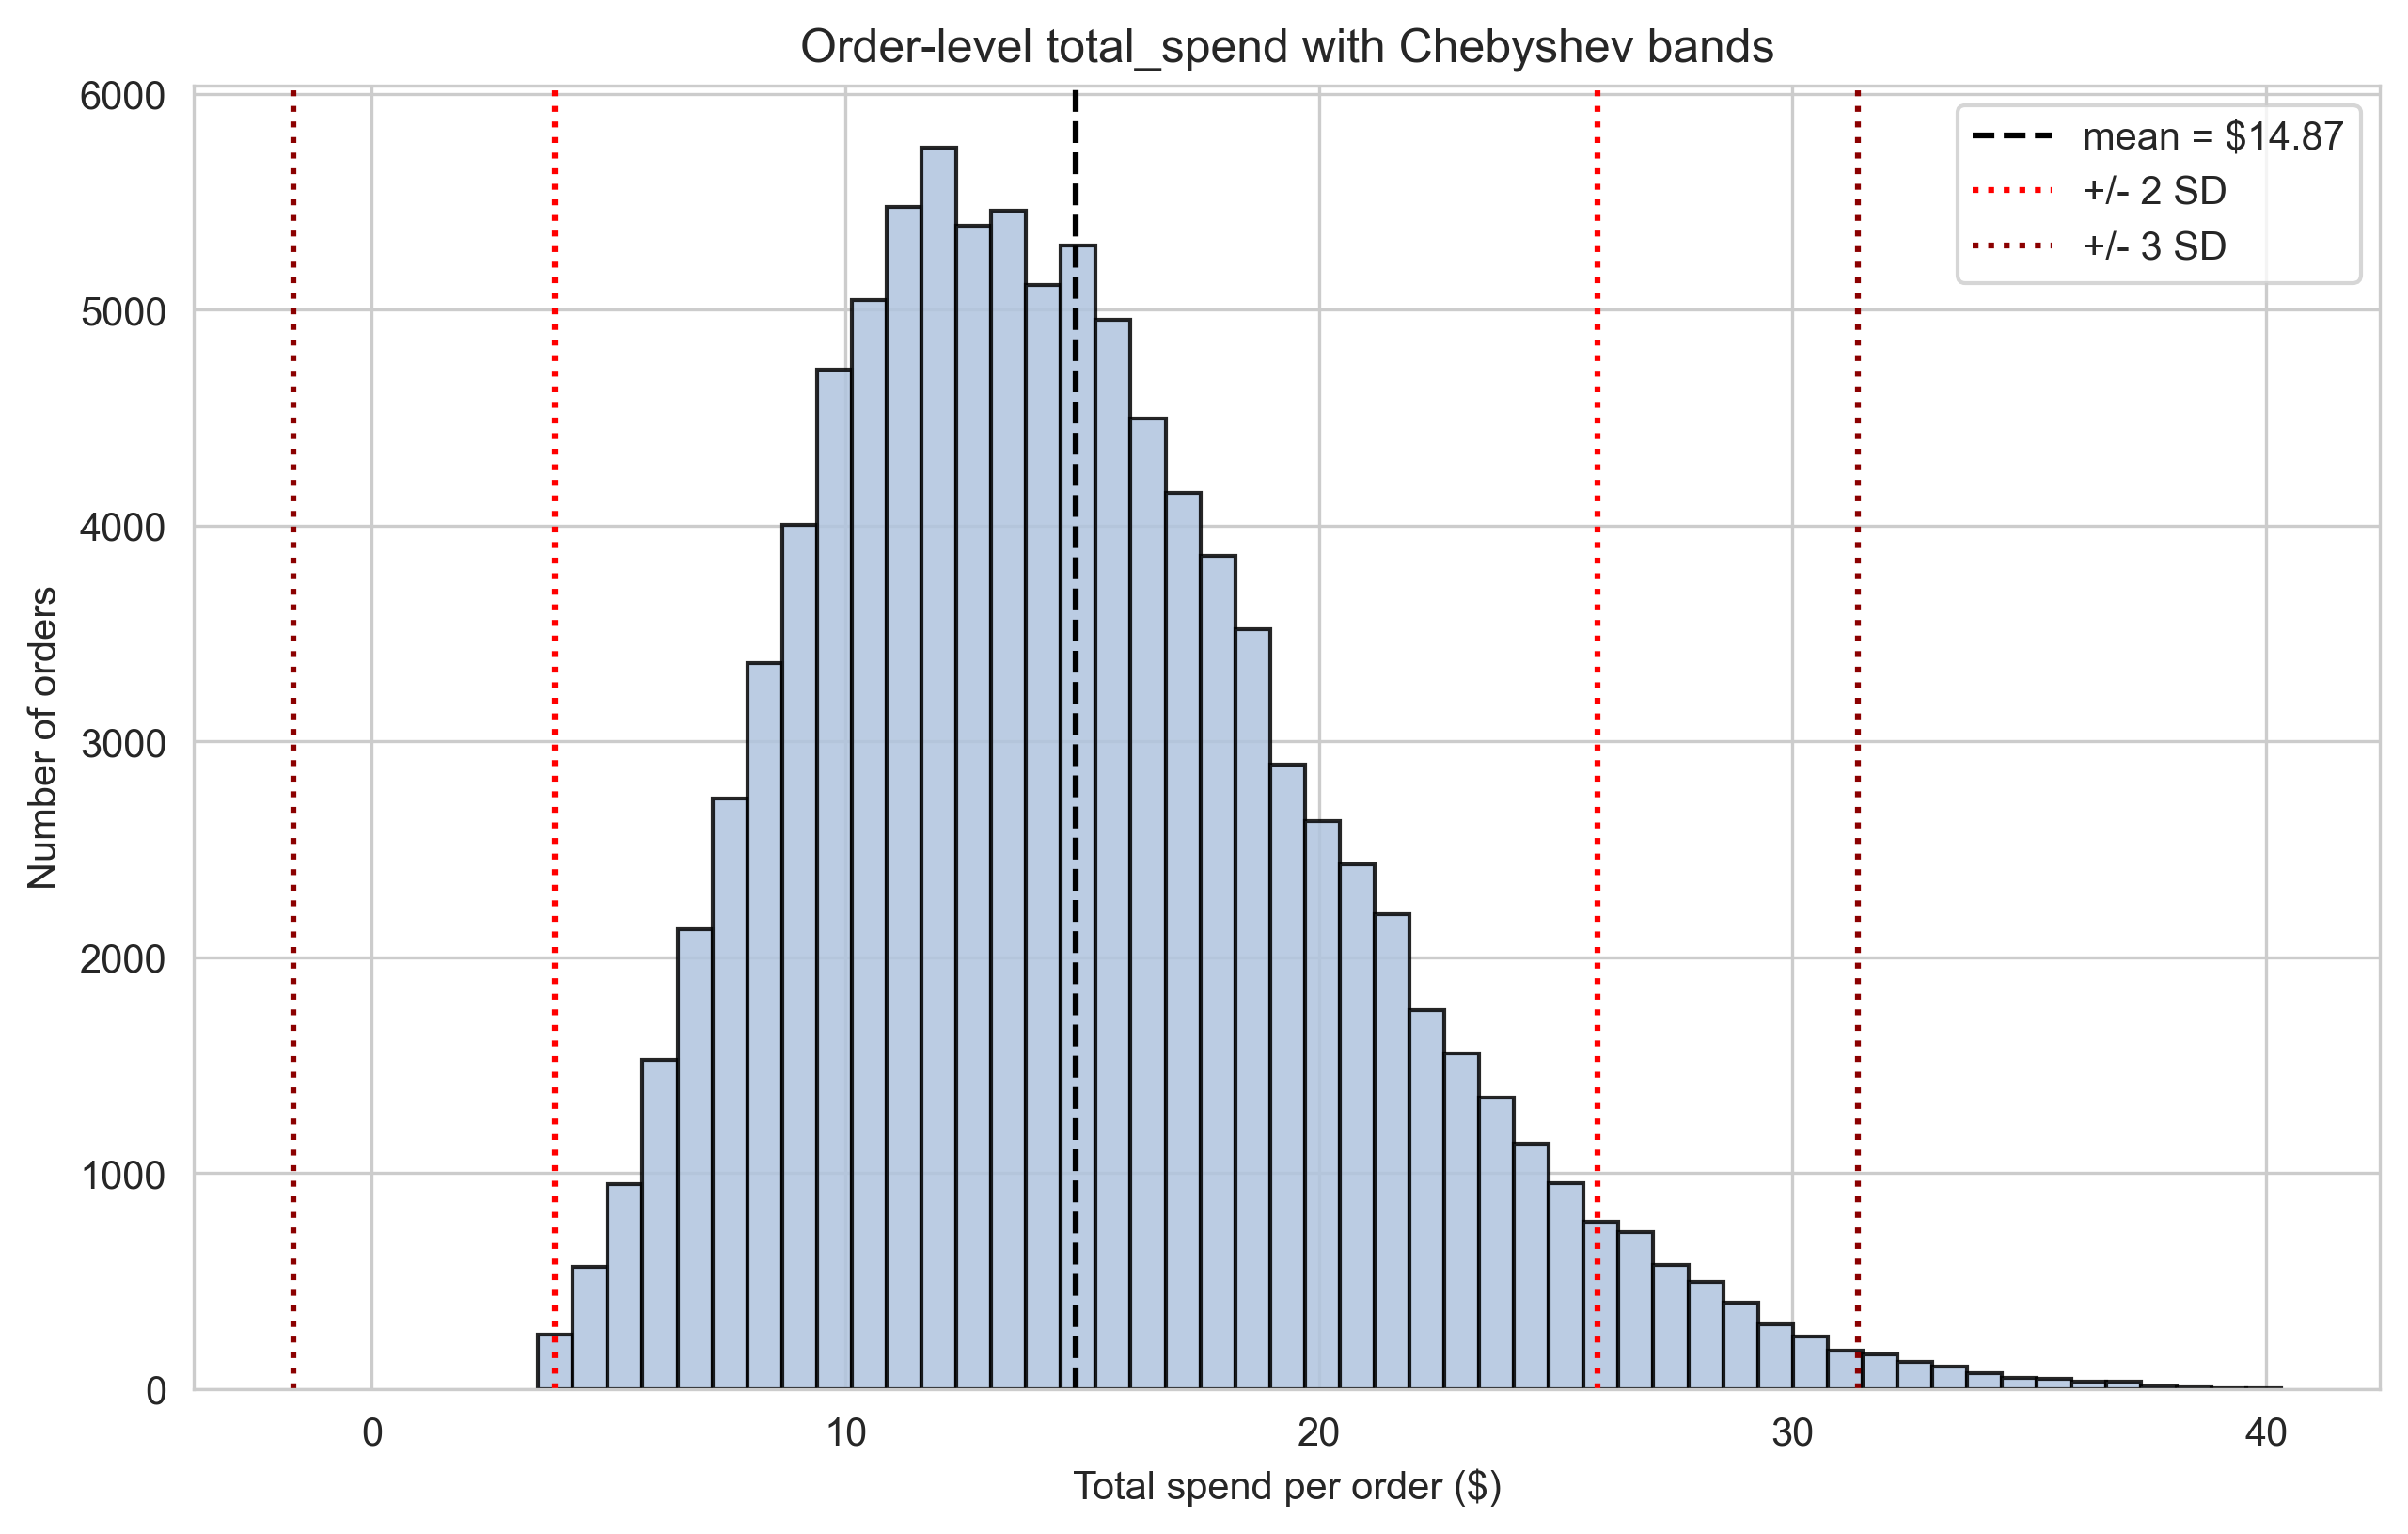
\includegraphics[width=0.95\columnwidth]{02_chebyshev_bands.png}
\caption{Histogram of total\_spend with mean and $\pm 2\sigma, \pm 3\sigma$ bands.}
\label{fig:cheb}
\end{figure}

A formal normality check (Figure~\ref{fig:normfit}) shows skewness $0.6701$, excess kurtosis $0.3775$, and a Shapiro\nobreakdash-Wilk statistic of $W=0.9734$ ($p\approx 1.6{\times}10^{-29}$) on a random subsample of size $5{,}000$. The body of the distribution is approximately normal but the right tail is heavier than normal. We therefore use empirical probabilities for tail events instead of the normal CDF.

\begin{figure}[!t]
\centering
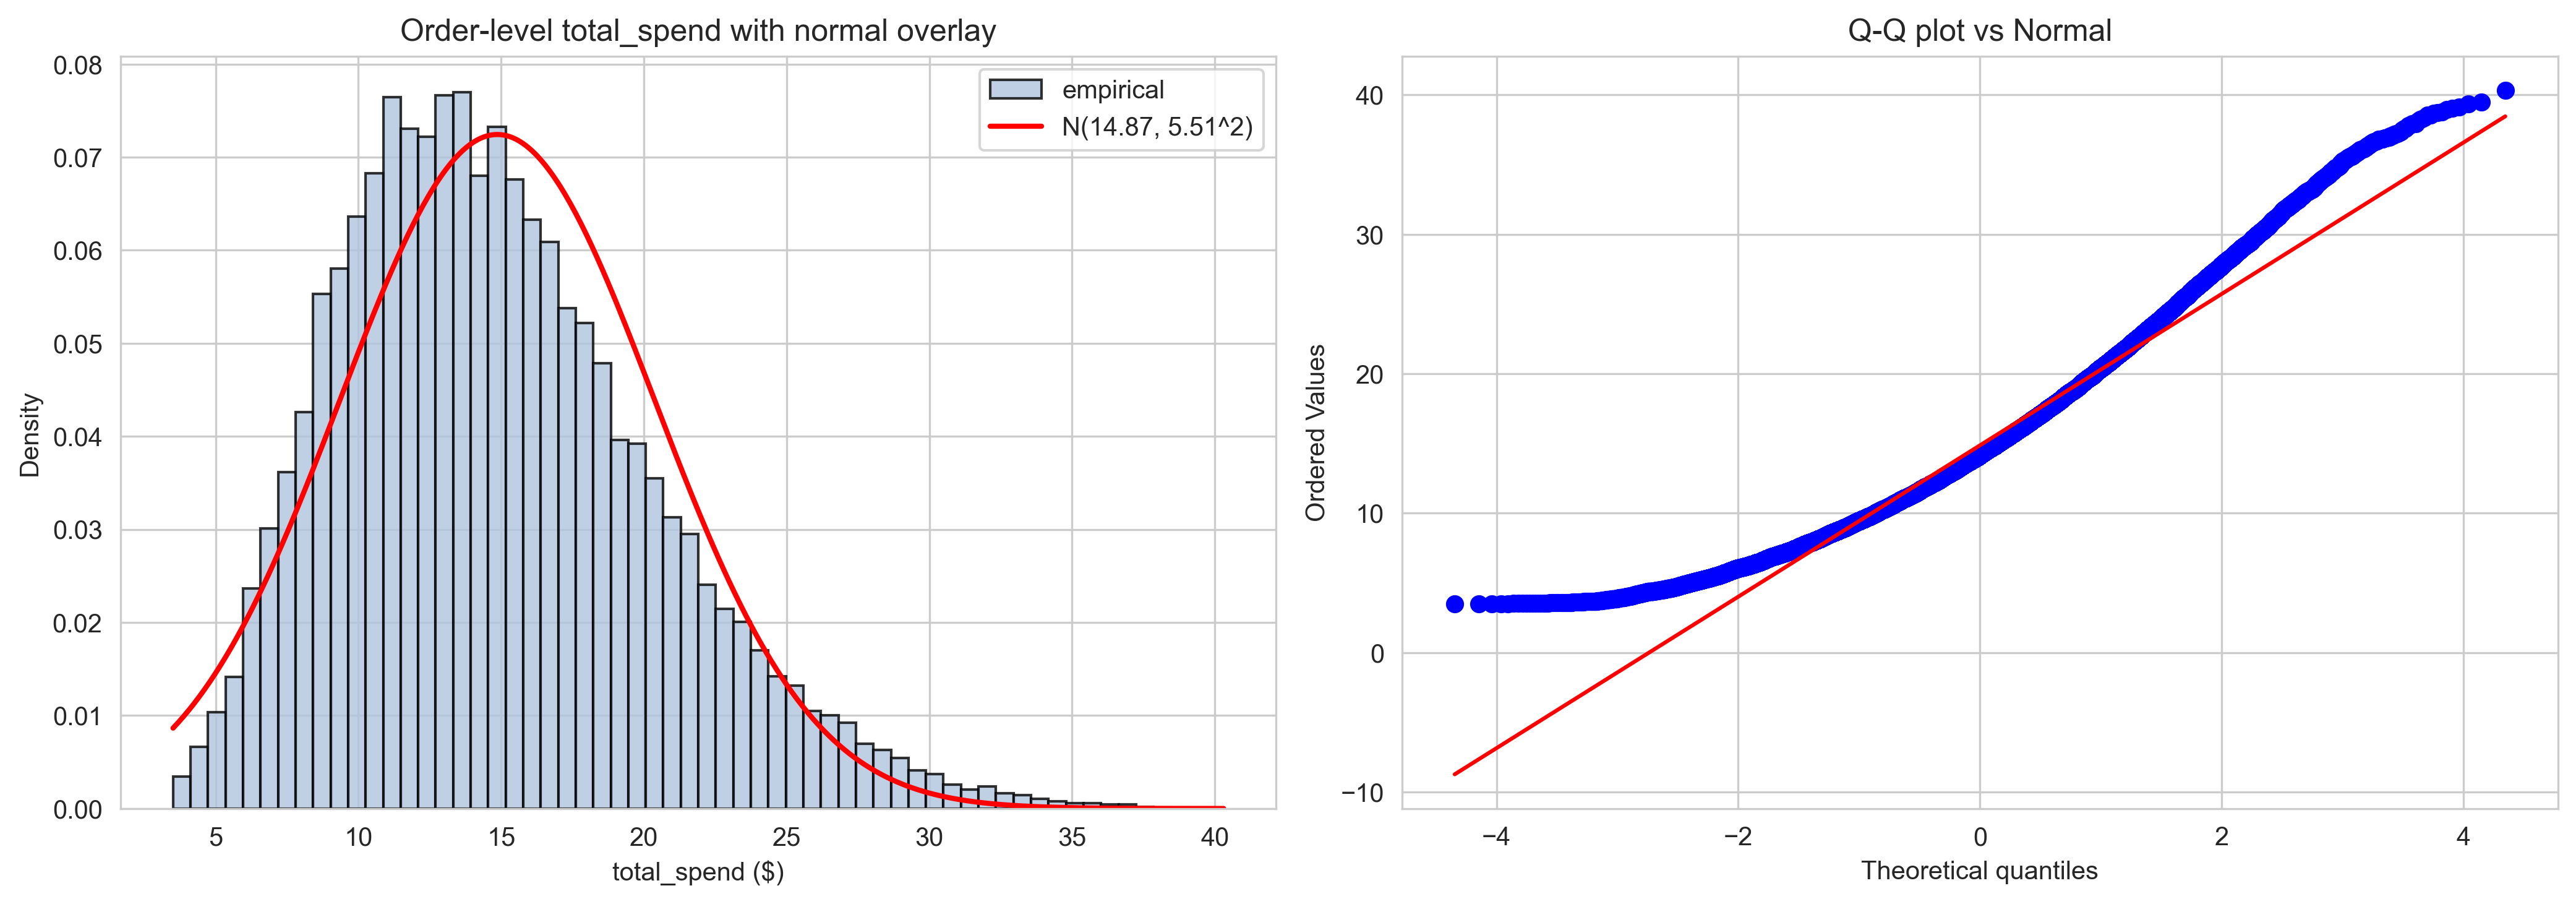
\includegraphics[width=\columnwidth]{02_normal_fit.png}
\caption{Histogram with normal overlay (left) and Q-Q plot vs normal (right) for total\_spend.}
\label{fig:normfit}
\end{figure}

\subsection{Confidence Intervals}
Applying (\ref{eq:ci}) at $\alpha=0.05$ gives an overall 95\% CI for the mean spend of $[\$14.83, \$14.90]$. Table~\ref{tab:ci} reports CIs by segment and Figure~\ref{fig:ci} visualizes them. The Mobile App segment is clearly separated from the other channels, and the rewards/non\nobreakdash-rewards CIs do not overlap.

\begin{table}[!t]
\caption{Selected 95\% Confidence Intervals for Mean \texttt{total\_spend}}
\label{tab:ci}
\centering
\renewcommand{\arraystretch}{1.1}
\begin{tabular}{lrrr}
\toprule
Segment & $n$ & Mean (\$) & 95\% CI (\$) \\
\midrule
Mobile App        & 42{,}521 & 18.08 & [18.02, 18.13] \\
Drive\nobreakdash-Thru        & 27{,}996 & 12.48 & [12.43, 12.53] \\
In\nobreakdash-Store Cashier  & 22{,}063 & 12.51 & [12.46, 12.57] \\
Kiosk             & 7{,}420  & 12.49 & [12.40, 12.58] \\
Rewards member    & 47{,}717 & 15.72 & [15.67, 15.77] \\
Non\nobreakdash-member        & 52{,}283 & 14.09 & [14.04, 14.13] \\
Age 18\nobreakdash-24         & 20{,}274 & 15.55 & [15.47, 15.63] \\
Age 55+           & 10{,}019 & 13.06 & [12.97, 13.15] \\
\bottomrule
\end{tabular}
\end{table}

\begin{figure}[!t]
\centering
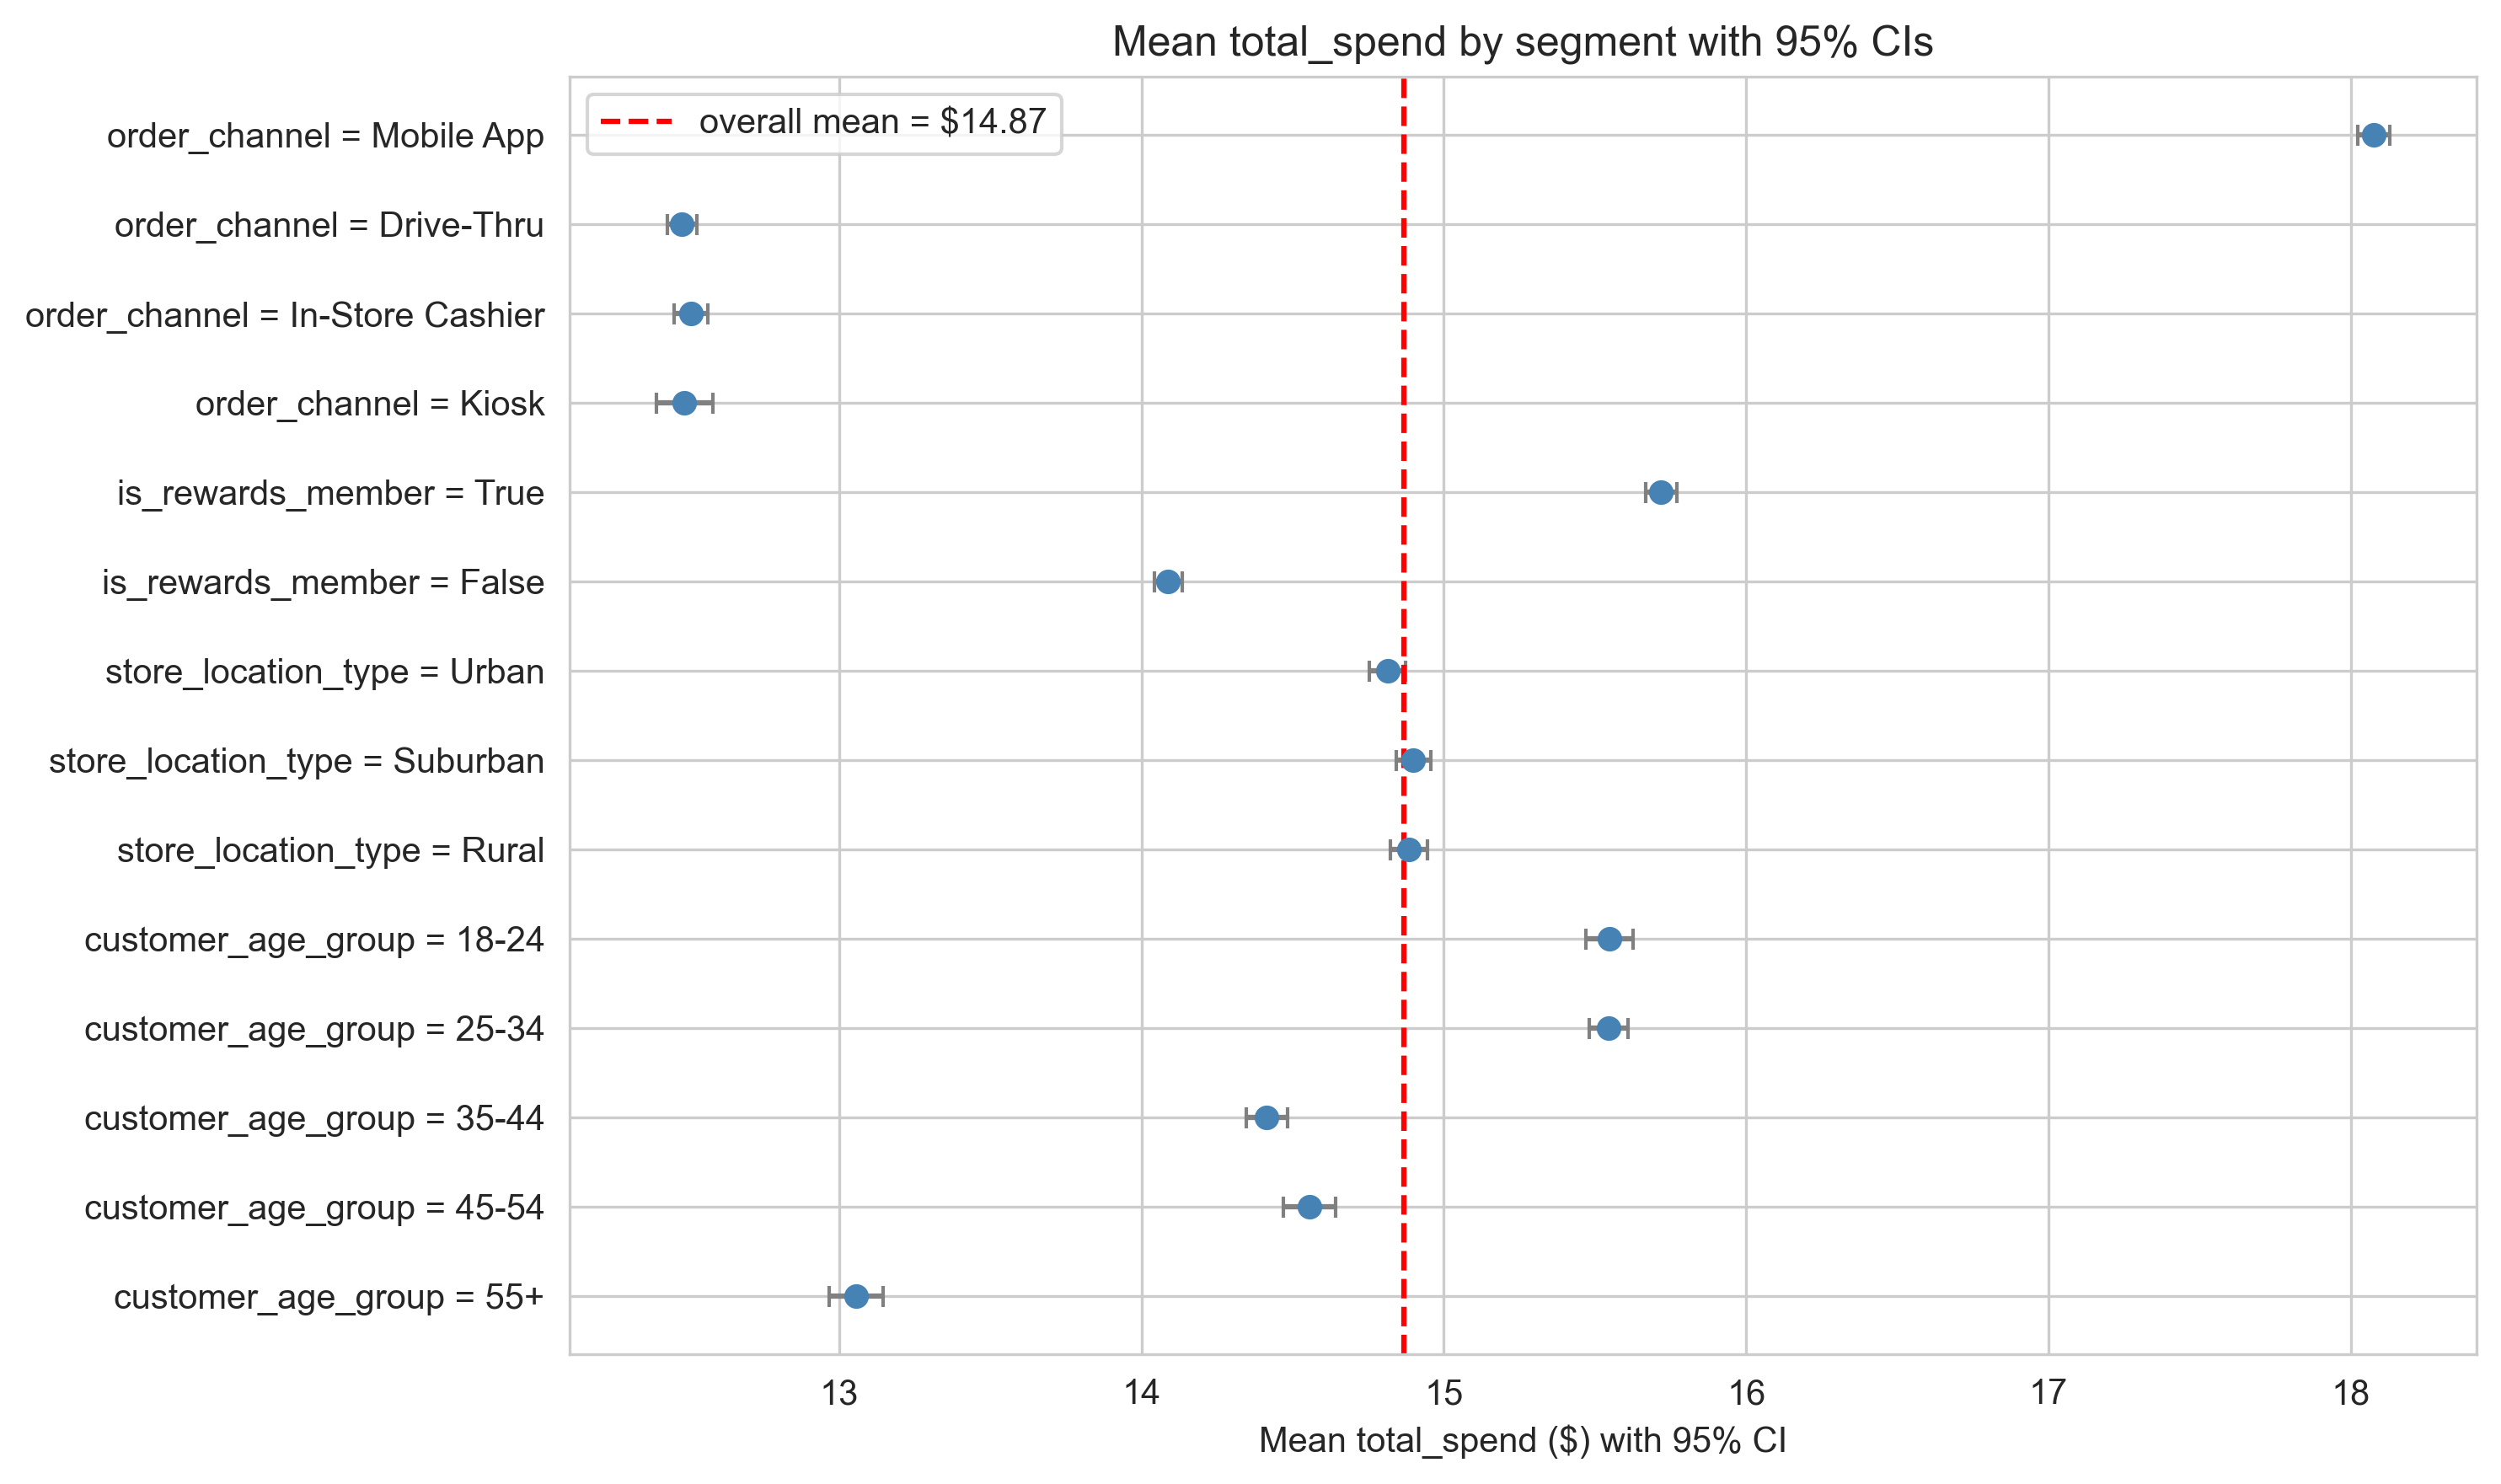
\includegraphics[width=\columnwidth]{03_ci_by_segment.png}
\caption{Mean total\_spend with 95\% confidence intervals by segment. The dashed red line is the overall mean.}
\label{fig:ci}
\end{figure}

\subsection{Hypothesis Tests}
We run four hypothesis tests at $\alpha=0.05$.

\textbf{Mobile vs non\nobreakdash-Mobile.} With $H_0:\mu_1=\mu_2$ and $H_a:\mu_1\ne\mu_2$, (\ref{eq:welch}) gives $\bar{x}_1-\bar{x}_2 = \$5.58$, $t=175.91$, and $p\approx 0$. The 95\% CI for the difference is $[\$5.52, \$5.65]$. We reject $H_0$.

\textbf{Rewards vs non\nobreakdash-rewards.} The same procedure gives $\bar{x}_1-\bar{x}_2 = \$1.63$, $t=47.08$, $p\approx 0$, and CI $[\$1.56, \$1.70]$. We reject $H_0$. The effect is small in dollars but the sample is large enough to detect it.

\textbf{Paired test, first vs latest order.} For the $14{,}857$ customers with at least two orders, (\ref{eq:paired}) gives $\bar{d}=\$0.05$, $t=0.77$, $p=0.44$, CI $[-\$0.07, \$0.17]$. We fail to reject $H_0$. There is no within\nobreakdash-customer drift in spend over the 24\nobreakdash-month window.

\textbf{High\nobreakdash-spender proportions.} Defining a high\nobreakdash-spender order as one with $\texttt{total\_spend}>\$20$ and applying (\ref{eq:zprop}), the rate is $0.2167$ for rewards and $0.1309$ for non\nobreakdash-rewards. The pooled $z=35.92$, $p\approx 0$, and the unpooled 95\% CI for the difference is $[0.0811, 0.0905]$. We reject $H_0$. Rewards membership is associated with a strictly higher tail rate, consistent with the mean test.

Figure~\ref{fig:tests} summarizes the three mean\nobreakdash-difference tests on a single axis.

\begin{figure}[!t]
\centering
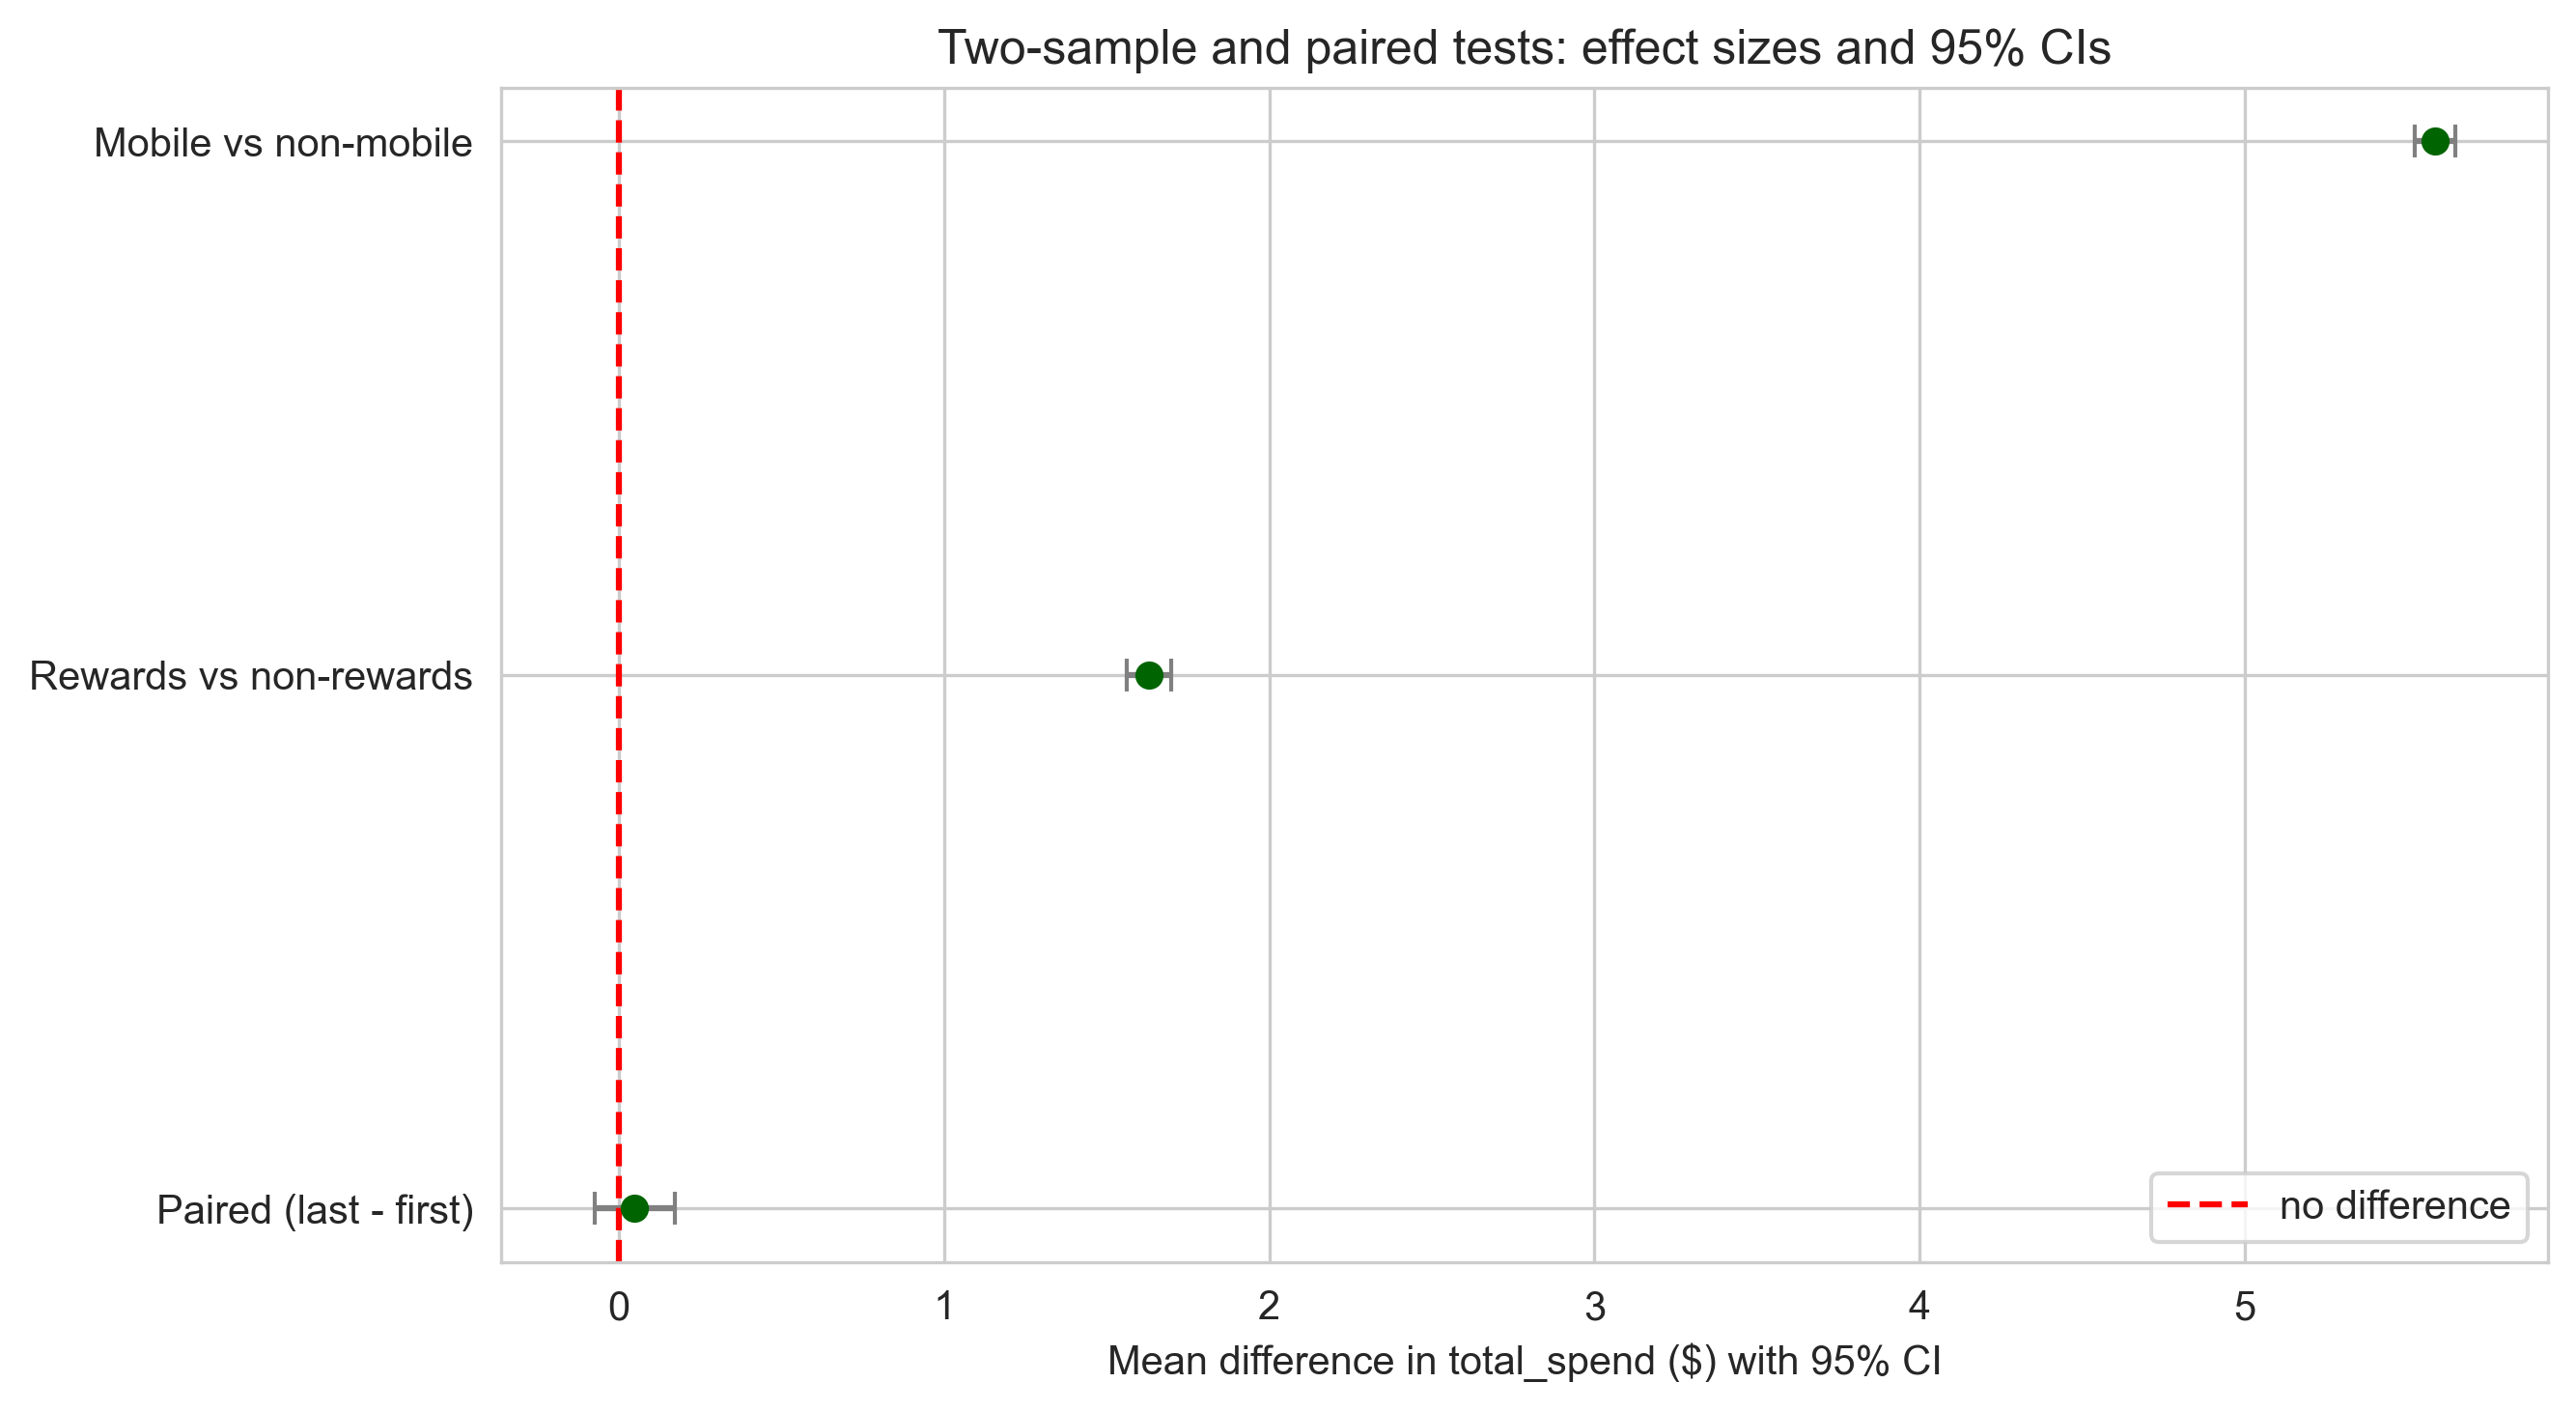
\includegraphics[width=\columnwidth]{03_test_effects.png}
\caption{Mean differences in total\_spend with 95\% CIs. The dashed red line is the no-difference reference.}
\label{fig:tests}
\end{figure}

\subsection{Empirical Probability and Bayes}
Empirical tail probabilities computed via (\ref{eq:emp}) appear in Table~\ref{tab:probs}. Figure~\ref{fig:empnorm} compares the empirical curve with a normal approximation that uses the sample $\mu$ and $\sigma$. The normal approximation overstates the share near the median (gap $-0.049$ at \$15) and understates the right tail (gap $+0.018$ at \$25, $+0.008$ at \$30, in absolute terms; in relative terms the underestimate is roughly $35\%$ and $72\%$). For tail questions we use the empirical numbers.

\begin{table}[!t]
\caption{Empirical vs Normal\nobreakdash-Approximation $P(\texttt{total\_spend}>t)$}
\label{tab:probs}
\centering
\renewcommand{\arraystretch}{1.1}
\begin{tabular}{rrrr}
\toprule
$t$ (\$) & $\hat{P}_{\text{emp}}$ & $\hat{P}_{\text{normal}}$ & Difference \\
\midrule
10 & 0.8054 & 0.8116 & $-0.006$ \\
15 & 0.4413 & 0.4904 & $-0.049$ \\
20 & 0.1718 & 0.1756 & $-0.004$ \\
25 & 0.0511 & 0.0329 & $+0.018$ \\
30 & 0.0107 & 0.0030 & $+0.008$ \\
\bottomrule
\end{tabular}
\end{table}

\begin{figure}[!t]
\centering
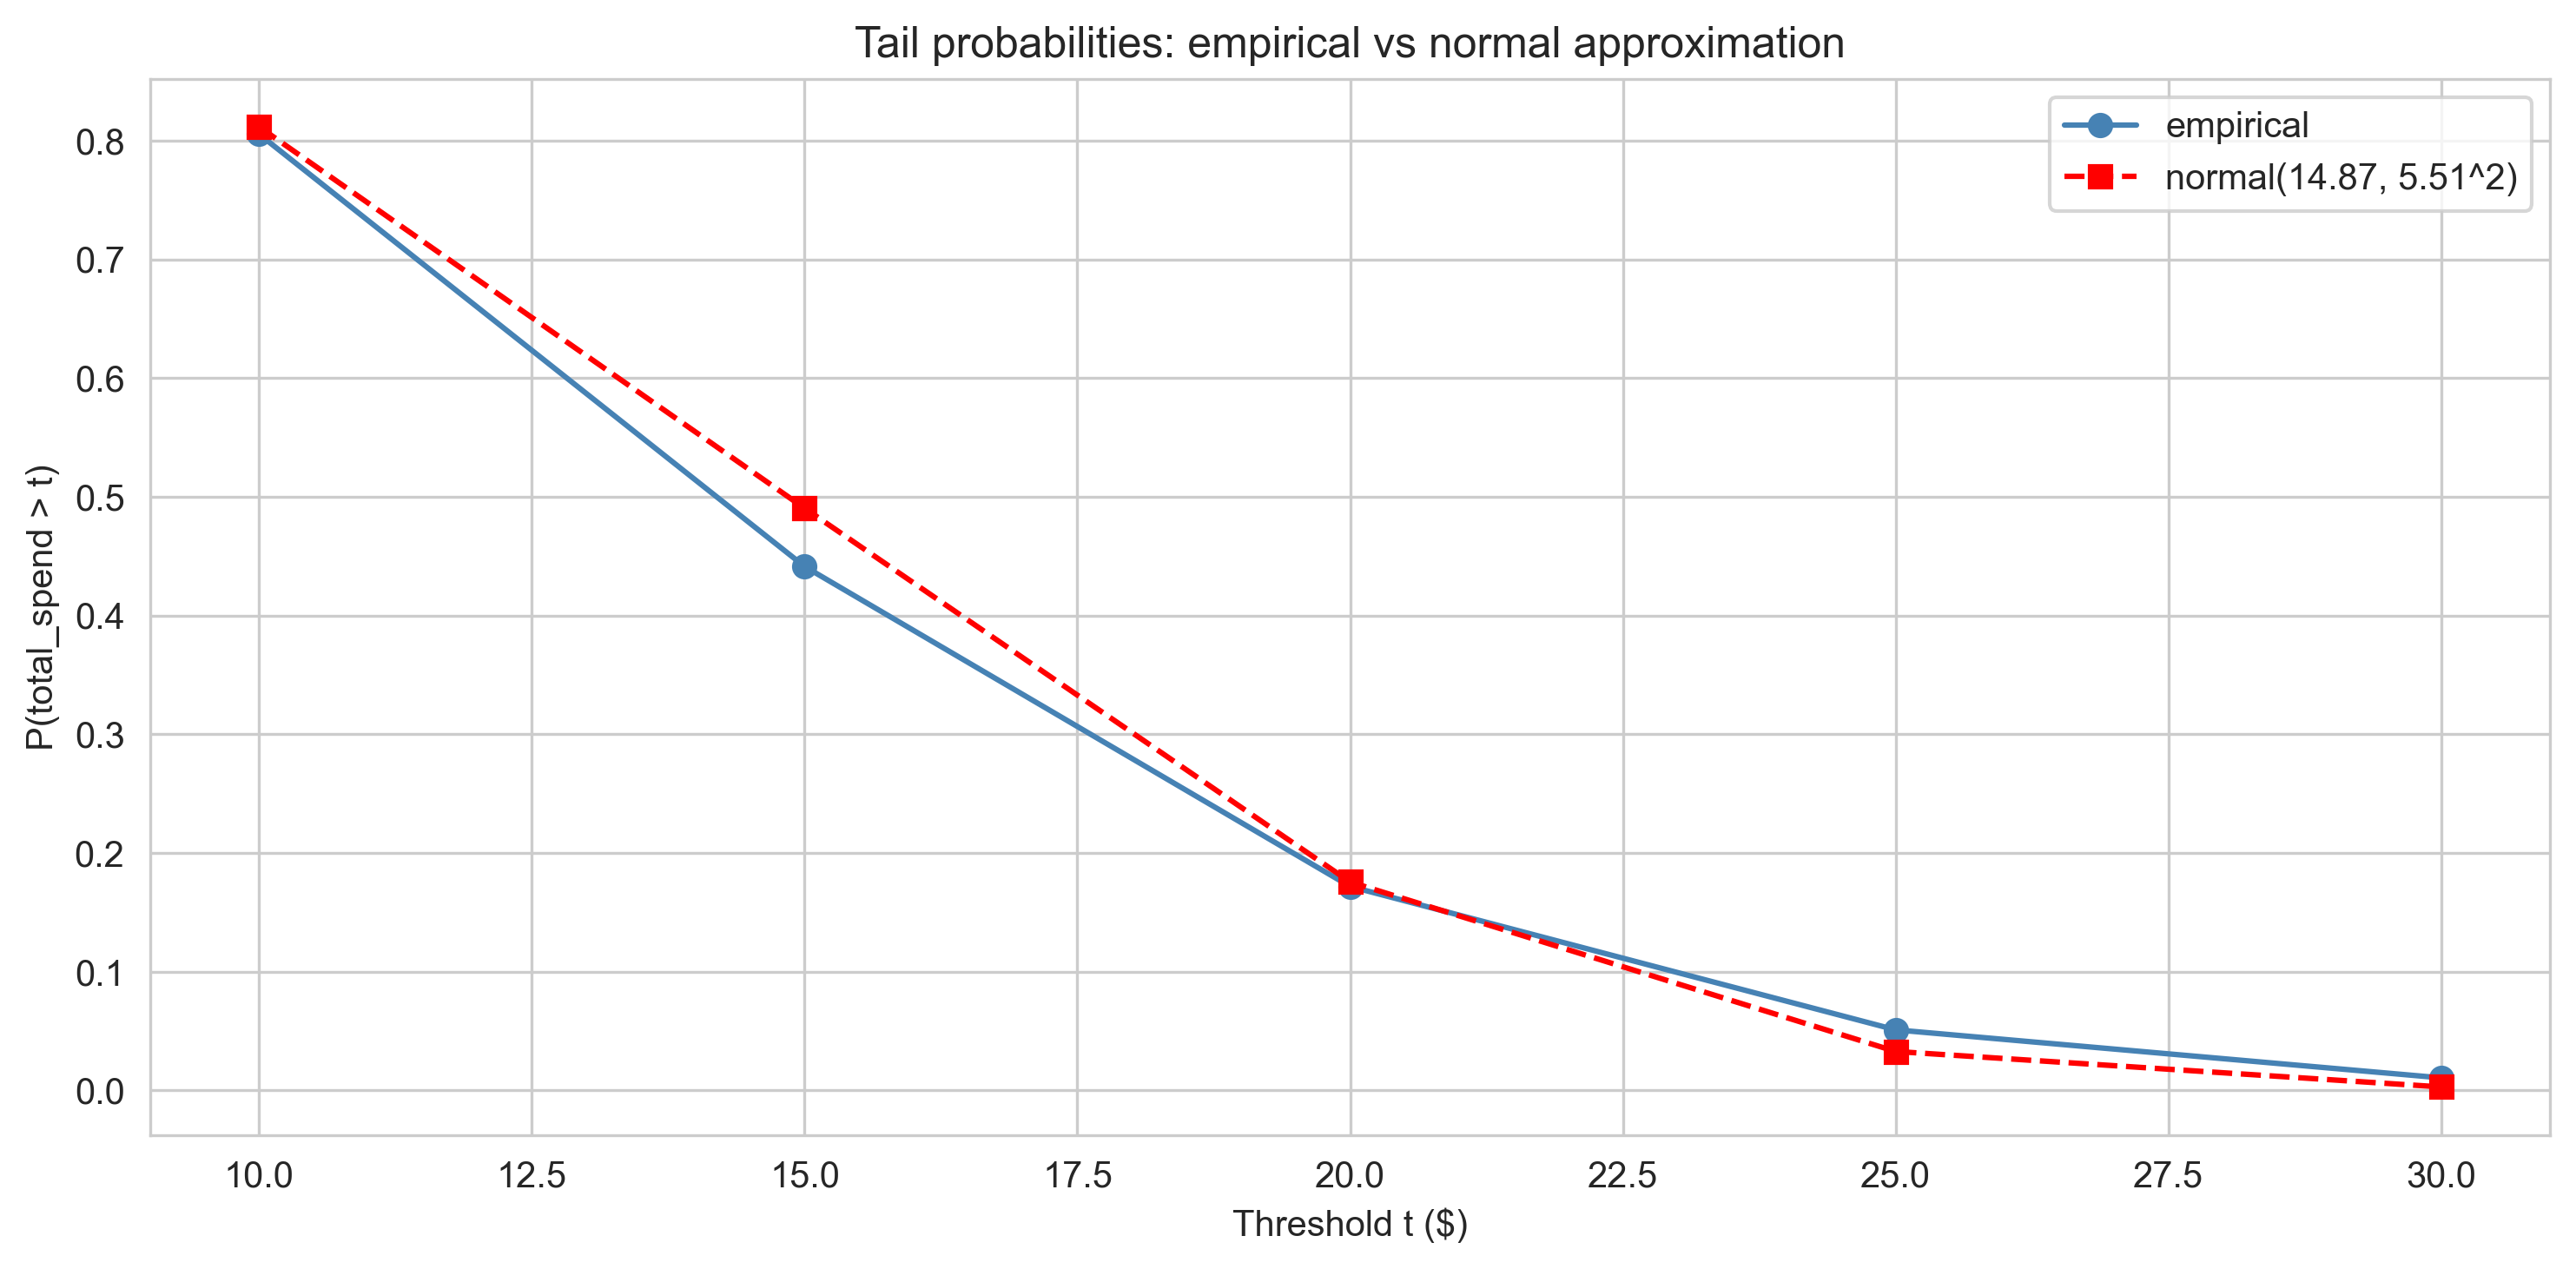
\includegraphics[width=0.95\columnwidth]{04_empirical_vs_normal.png}
\caption{Tail probabilities $P(\mathrm{total\_spend}>t)$: empirical vs normal approximation.}
\label{fig:empnorm}
\end{figure}

Conditional probabilities of a high\nobreakdash-spender order ($>\$25$) are shown in Figure~\ref{fig:cond}. By channel, $P(\text{spend}>25\mid\text{Mobile})=0.1127$ versus about $0.005$ for the other three channels, a $\approx 20{\times}$ ratio. By rewards, $P(\text{spend}>25\mid\text{Rewards})=0.0672$ versus $0.0364$, a $\approx 1.85{\times}$ ratio.

\begin{figure}[!t]
\centering
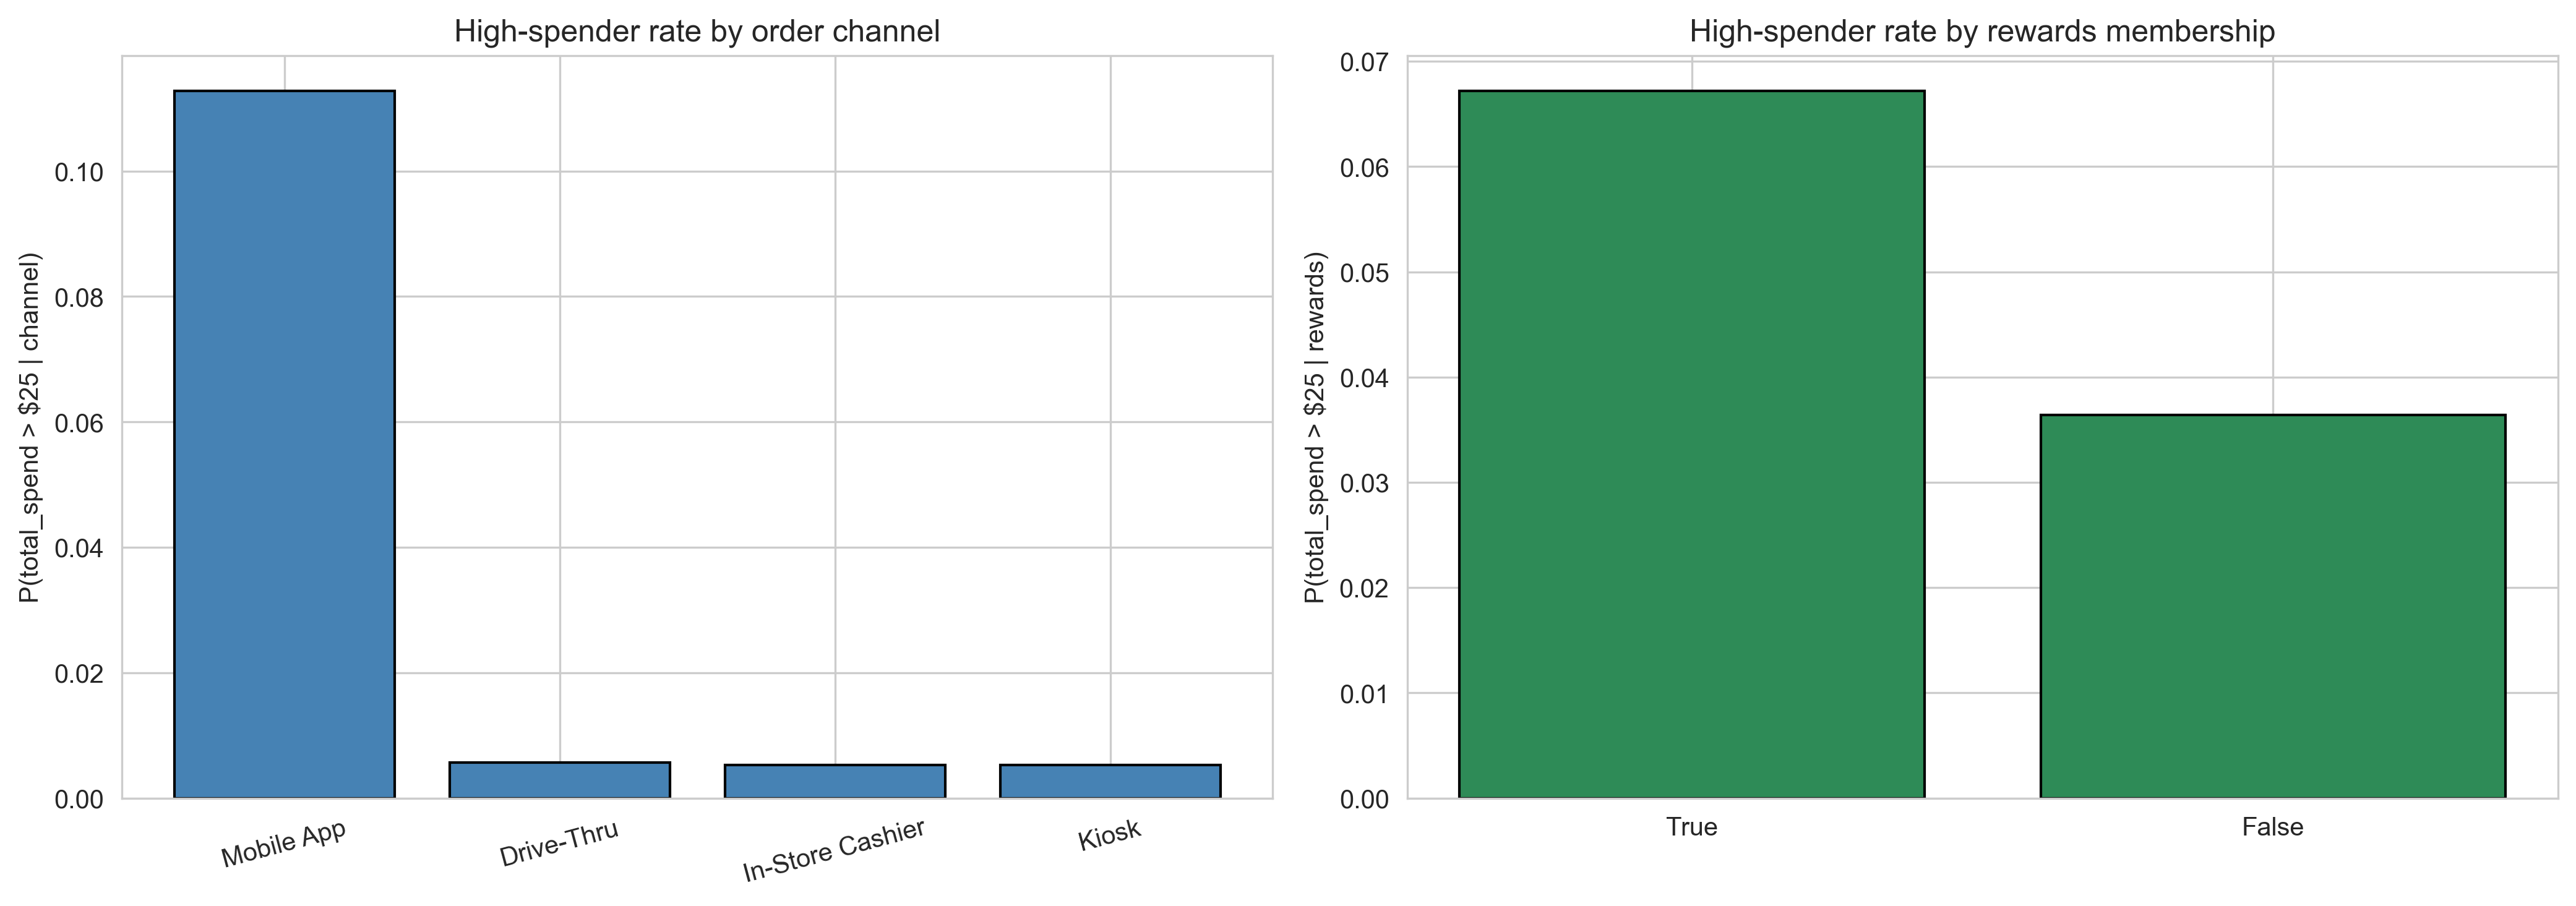
\includegraphics[width=\columnwidth]{04_conditional_probs.png}
\caption{Conditional high-spender probabilities by channel and rewards membership.}
\label{fig:cond}
\end{figure}

Applying Bayes' theorem (\ref{eq:bayes}) with $A=\{\text{Mobile App}\}$ and $B=\{\text{spend}>25\}$:
\[
P(A\mid B) = \frac{0.1127 \cdot 0.4252}{0.1127 \cdot 0.4252 + 0.0055 \cdot 0.5748} = 0.9385.
\]
A direct count gives $0.9385$, confirming the chain. Almost all high\nobreakdash-spender orders come from the Mobile App. The same procedure on rewards gives $P(\text{Rewards}\mid\text{spend}>25)=0.6274$.

\subsection{Random Variable: Cart Size}
\texttt{cart\_size} is a discrete random variable on $\{1,\dots,10\}$. The empirical PMF (Figure~\ref{fig:pmf}) is concentrated on $3$ to $5$ with a right tail to $10$. Applying (\ref{eq:rv}) gives $E[X]=3.7415$ and $\mathrm{Var}(X)=2.8826$, matching the descriptive moments in Table~\ref{tab:desc}.

\begin{figure}[!t]
\centering
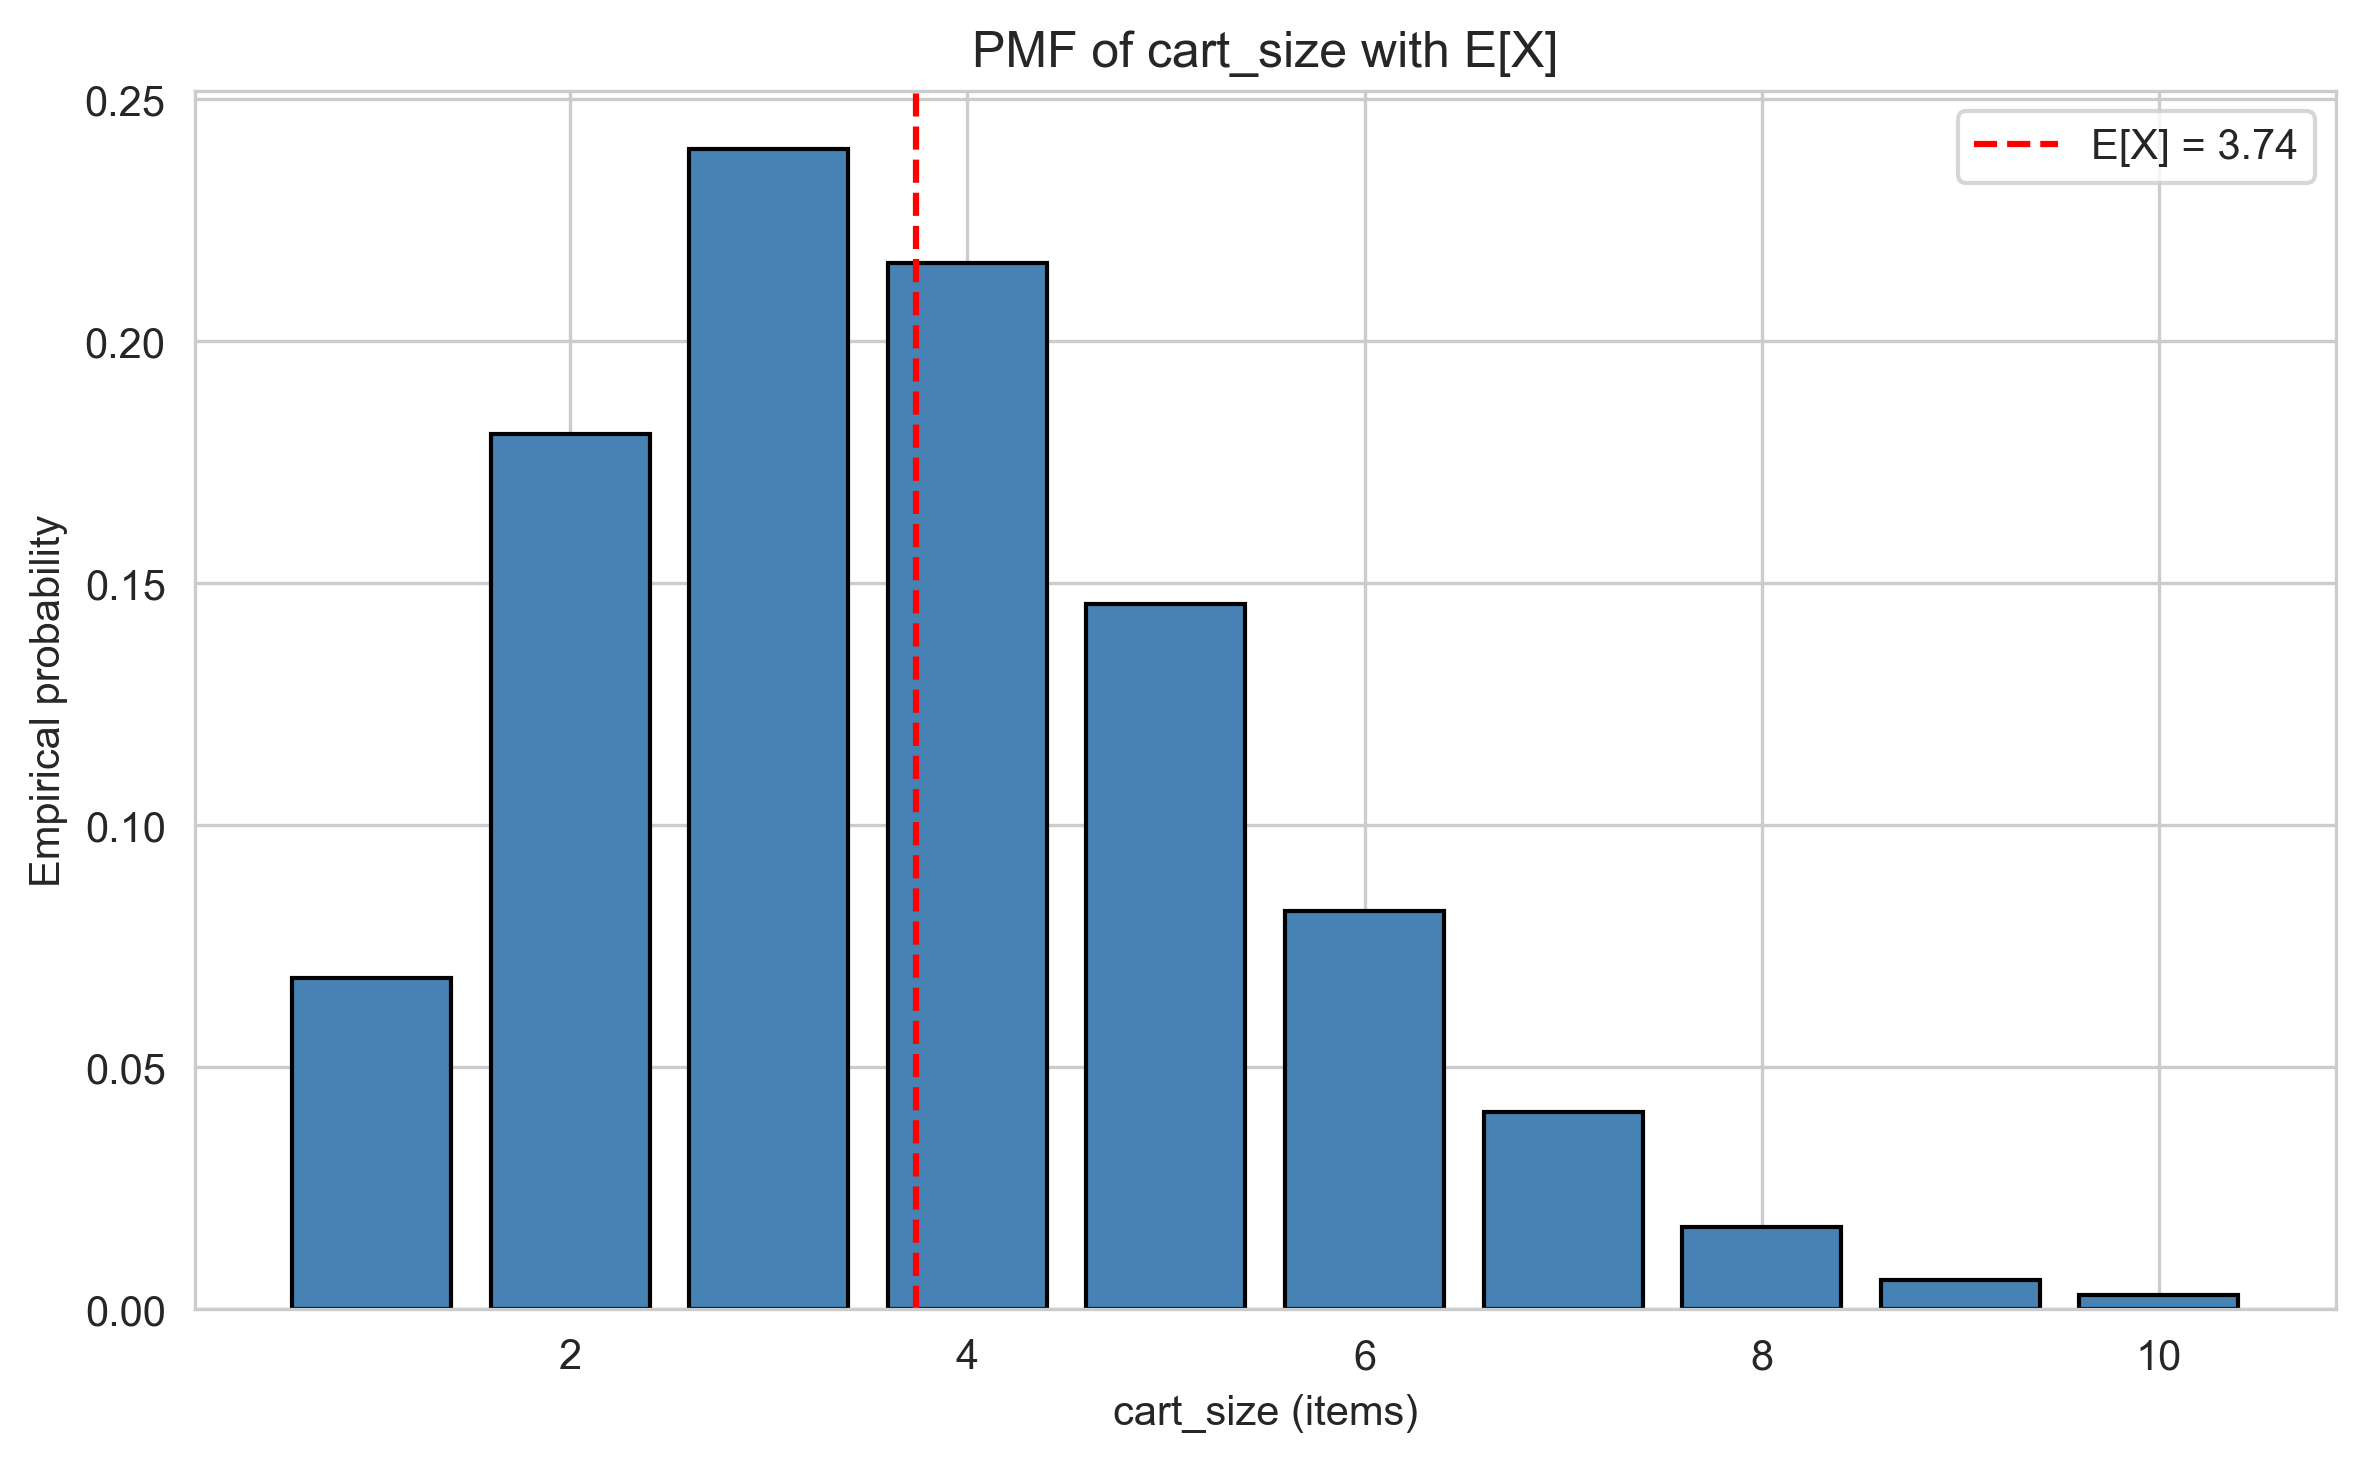
\includegraphics[width=0.95\columnwidth]{04_pmf_cart_size.png}
\caption{Empirical PMF of cart\_size with $E[X]$ marked.}
\label{fig:pmf}
\end{figure}

\subsection{Linear Model via Normal Equations and Gradient Descent}
\label{sec:linmodel}
We fit
\[
\begin{aligned}
y_i &= \beta_0 + \beta_1\,\texttt{cart}_i
      + \beta_2\,\texttt{custom}_i \\
    &\quad + \beta_3\,\mathbf{1}\{\text{Mobile}_i\}
      + \varepsilon_i .
\end{aligned}
\]
The design matrix is $X\in\mathbb{R}^{100000\times 4}$ with a leading column of ones. Solving the normal equations (\ref{eq:normal}) gives
\[
\hat{\beta} = (2.156,\;2.685,\;0.924,\;2.331).
\]
The condition number of $X^{\top}X$ is $1.54{\times}10^{2}$, well within the safe range. The model fit summary on the full sample is $\mathrm{RSS}=150{,}098$, $\mathrm{TSS}=3{,}032{,}454$, $R^2=0.9505$, and residual standard error $\hat{\sigma}=\$1.23$. Diagnostics in Figure~\ref{fig:diag} are well\nobreakdash-behaved with a roughly bell\nobreakdash-shaped residual distribution and no obvious systematic pattern.

\begin{figure}[!t]
\centering
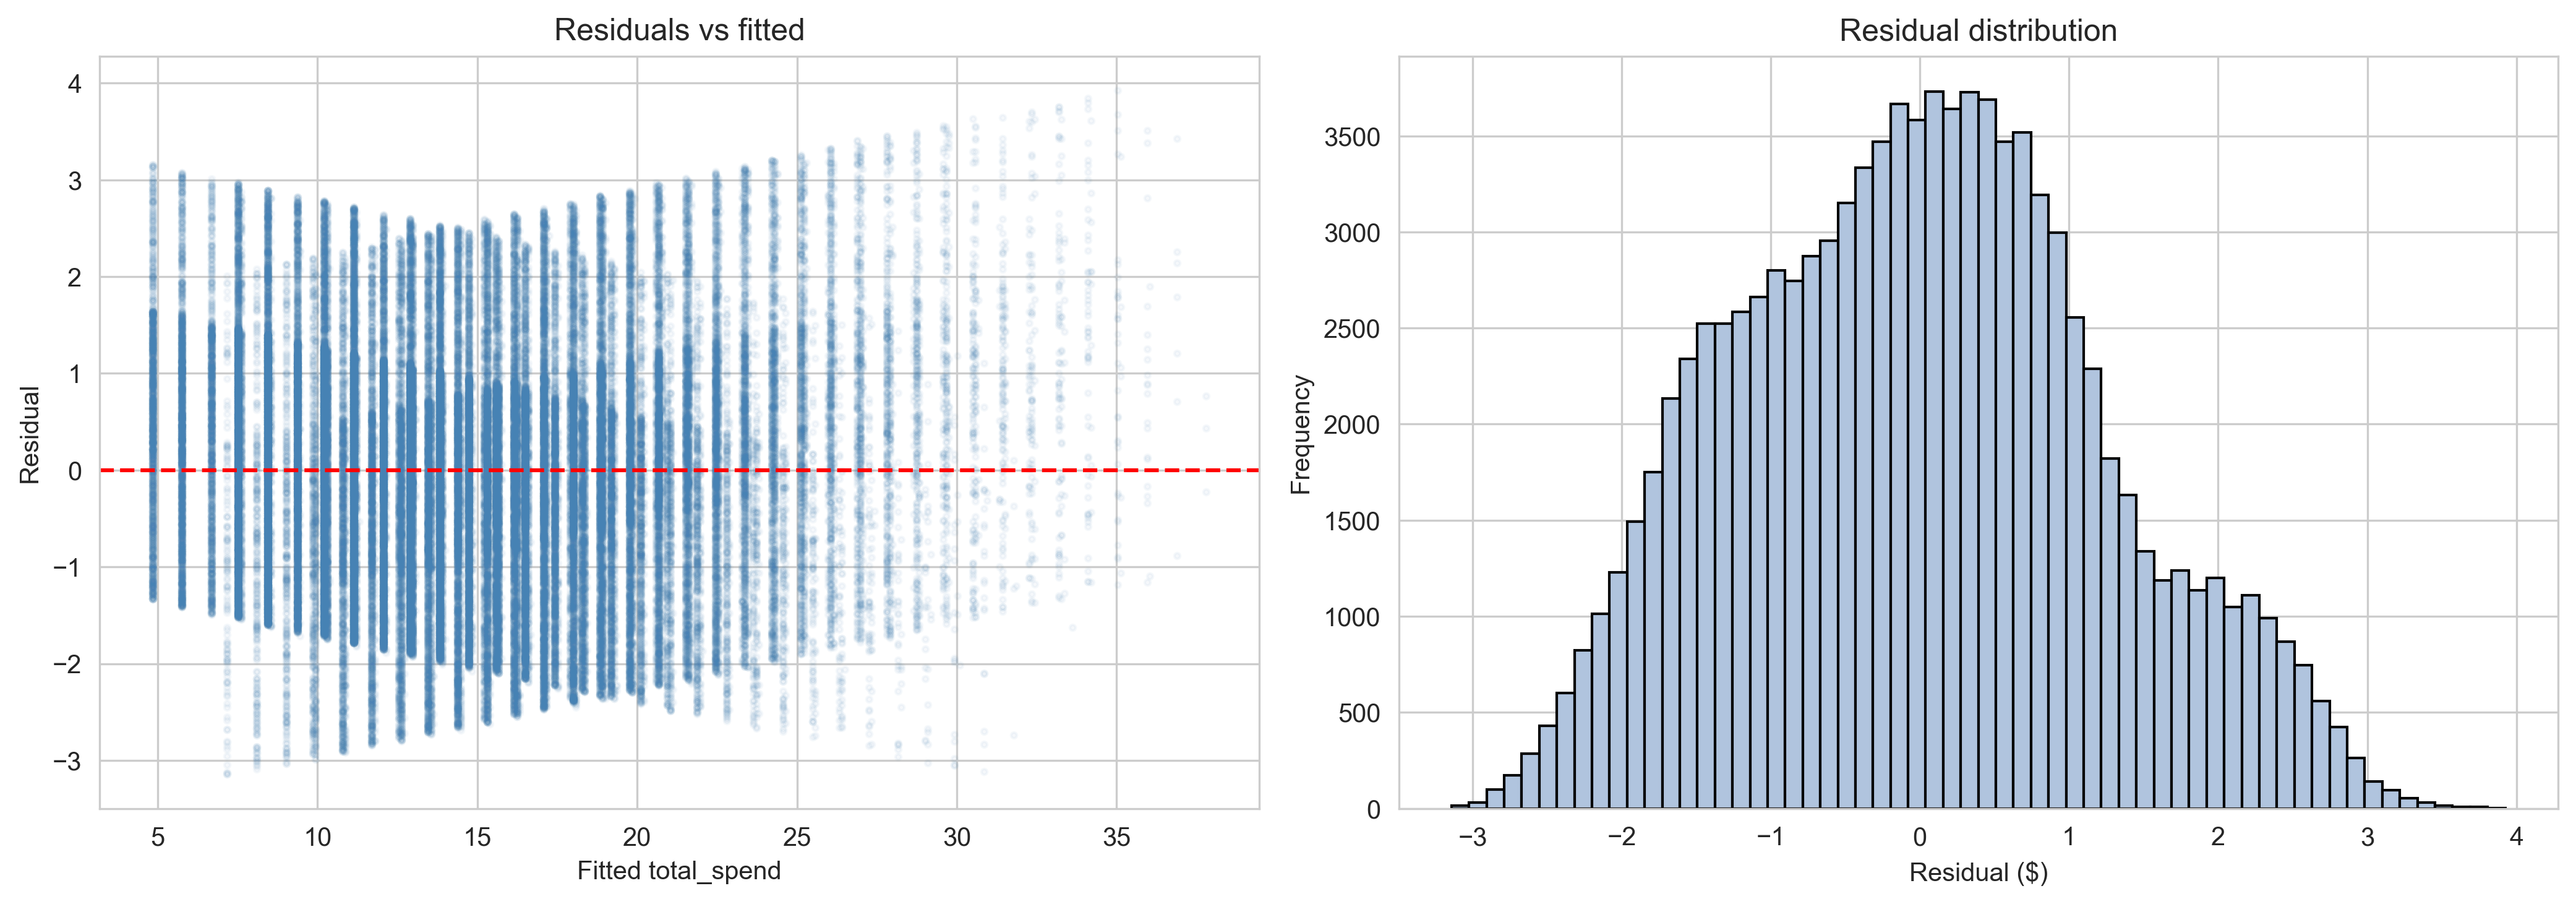
\includegraphics[width=\columnwidth]{05_lm_diagnostics.png}
\caption{Linear model diagnostics: residuals vs fitted values (left) and residual histogram (right).}
\label{fig:diag}
\end{figure}

\textbf{Optimization view.} Standardizing the predictors and running gradient descent (\ref{eq:gd}) from $\beta=0$ at learning rate $0.05$ converges to the same coefficients in $5{,}000$ steps, with L2 distance $0$ to the closed\nobreakdash-form solution. Figure~\ref{fig:gd} shows the loss curve. This connects Lecture 9 (calculus and optimization) to Lectures 10 and 11 (linear algebra and systems of linear equations).

\begin{figure}[!t]
\centering
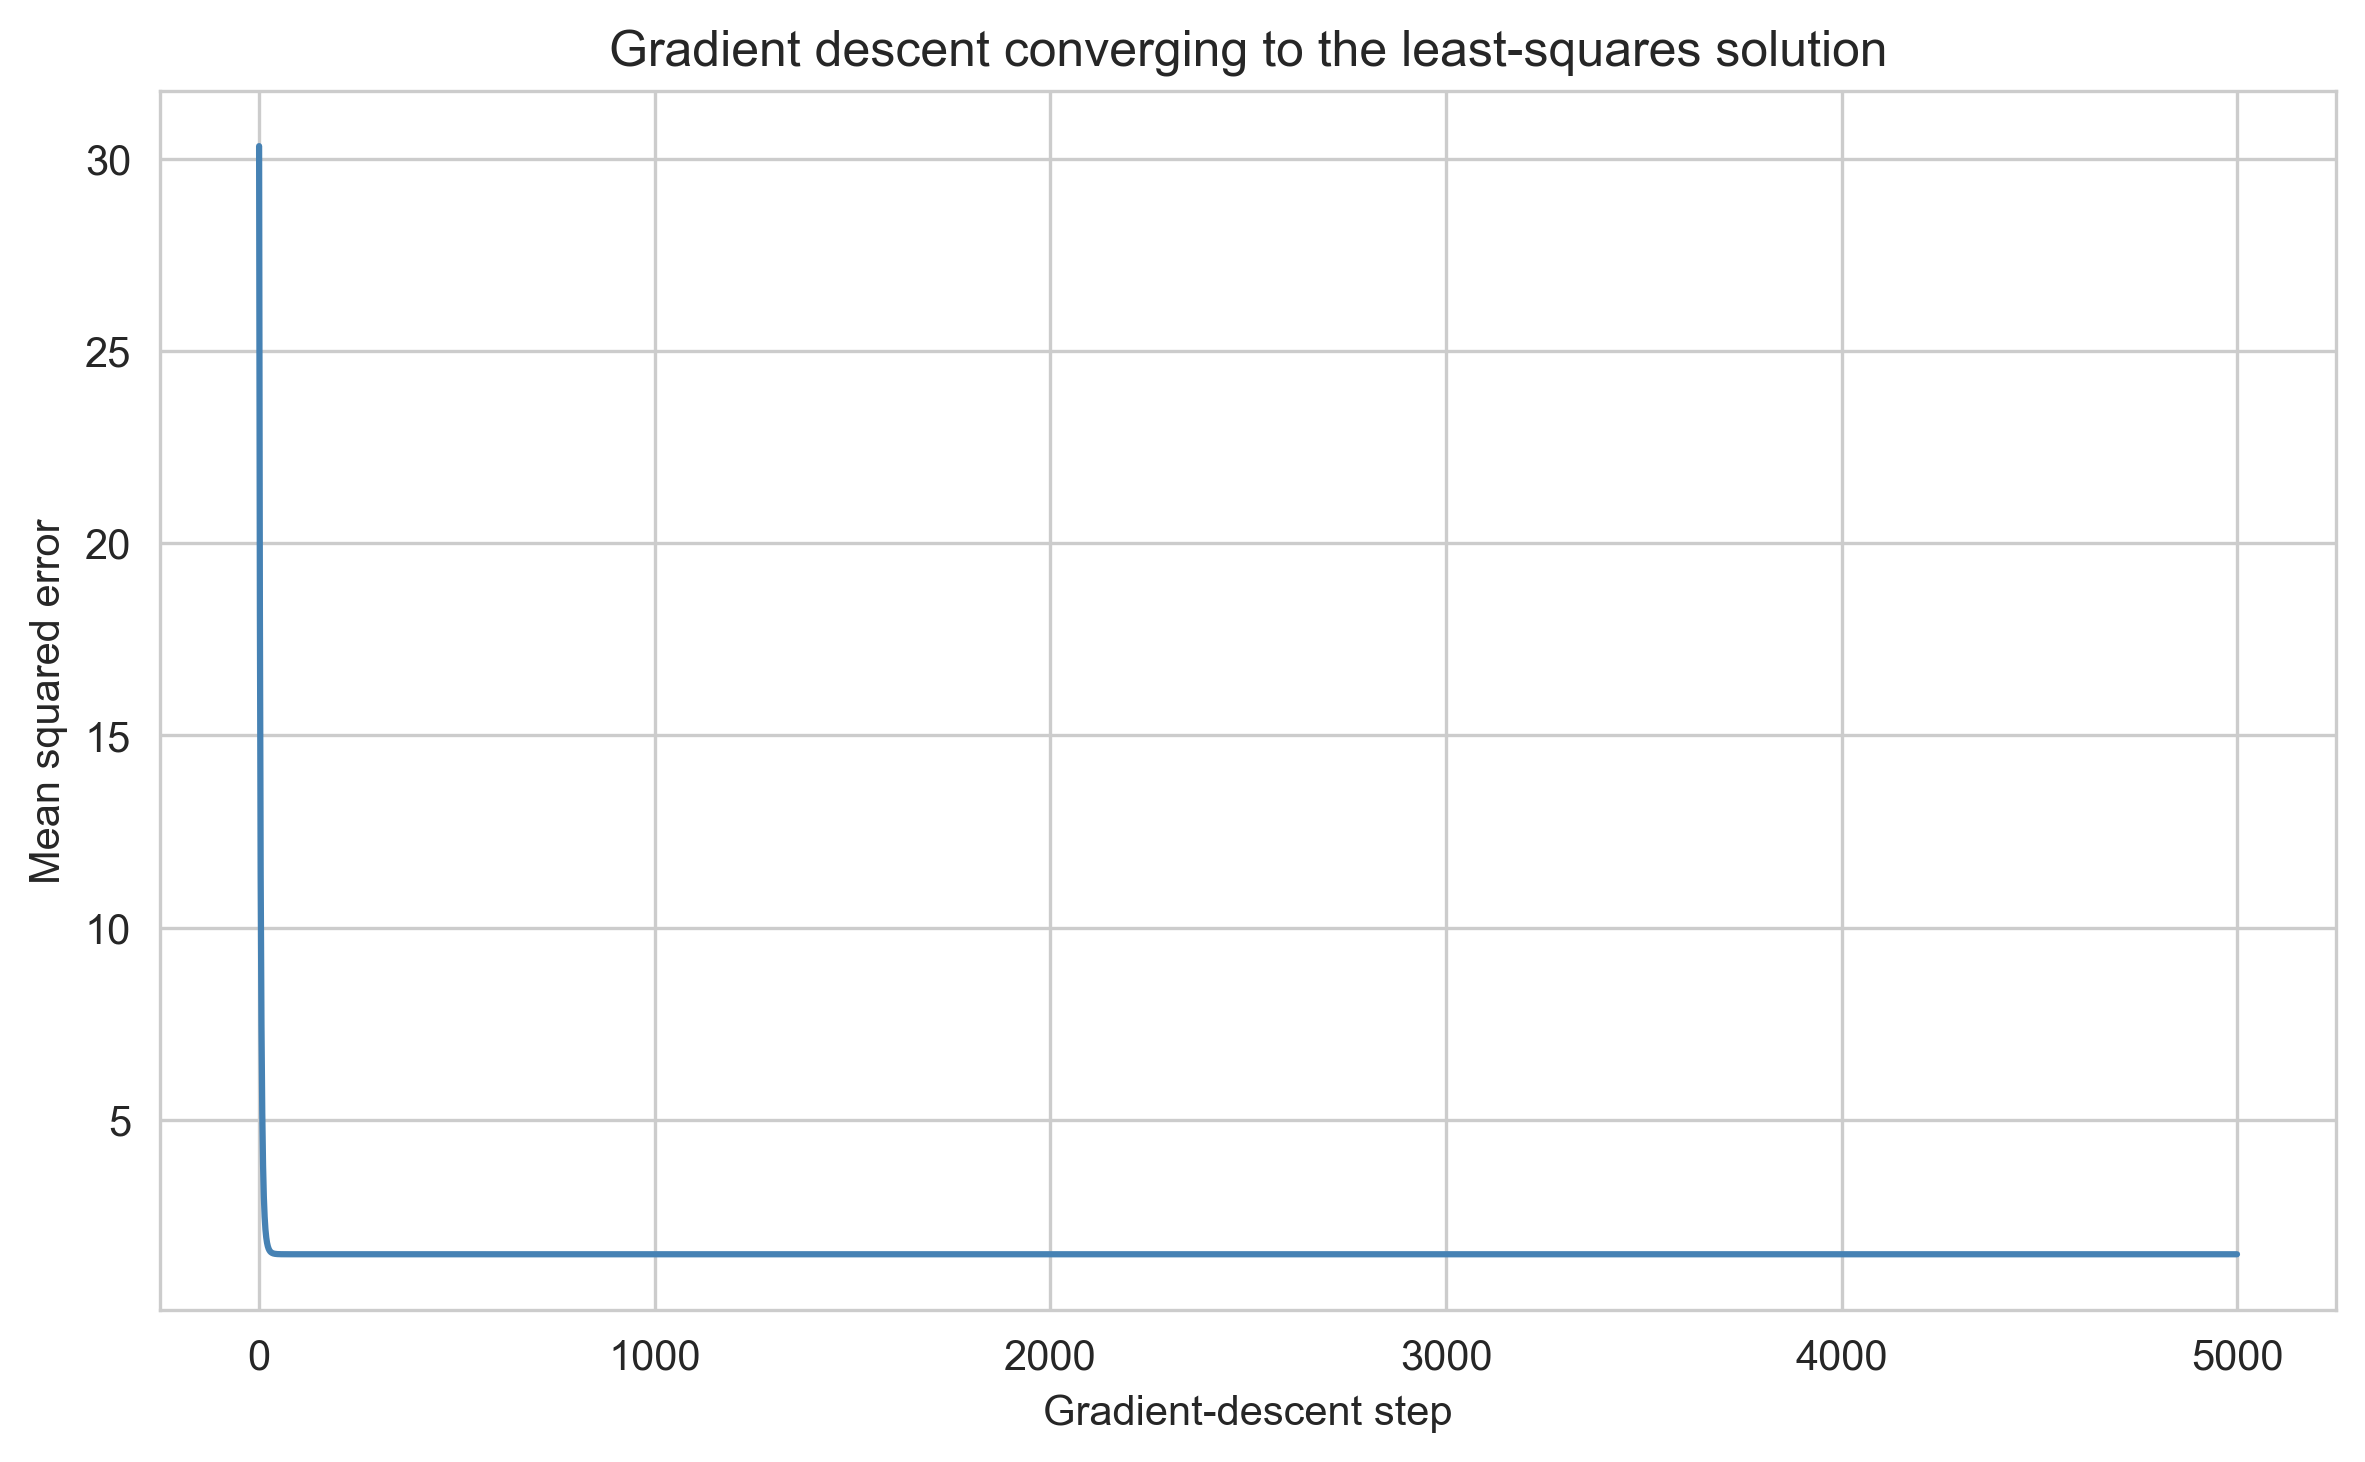
\includegraphics[width=0.85\columnwidth]{05_gd_convergence.png}
\caption{Gradient descent on the standardized least-squares loss converges to the closed-form solution.}
\label{fig:gd}
\end{figure}

\section{Discussion and Interpretation}

\subsection{What the Numbers Mean for the Business}
The Mobile App channel is the single largest revenue lever in the data. Mobile orders average \$5.58 more than non\nobreakdash-Mobile orders, and even after controlling for cart size and customizations the channel premium is still \$2.33 per order. The conditional and Bayesian analysis tells the same story from a different angle: about 94\% of orders above \$25 are placed through the Mobile App. Rewards membership matters but in a smaller way ($\$1.63$ per order on average, $1.85{\times}$ higher tail rate). Within a customer's history, the first and latest order do not differ on average, so observed cross\nobreakdash-segment differences are between\nobreakdash-segment effects rather than within\nobreakdash-customer drift.

\subsection{Cross-Method Consistency}
The same conclusions show up under multiple methods. The mean test, the proportion test on the right tail, and the Bayesian posterior all point to Mobile being the dominant high\nobreakdash-spender segment. The linear model splits credit between cart size, customizations, and Mobile in a way that is consistent with the order\nobreakdash-level correlations: the strongest predictor by correlation also has the largest standardized coefficient.

\subsection{Deployment}
Translating the analysis into a production setting at Starbucks scale would proceed in three layers. (i) \emph{Batch refresh}: a daily or hourly job recomputes the descriptive statistics, segment means and CIs, and updates the linear model coefficients. The closed\nobreakdash-form $\hat{\beta}=(X^{\top}X)^{-1}X^{\top}y$ is cheap when $p$ is small and $n$ is large because $X^{\top}X\in\mathbb{R}^{p\times p}$ does not grow with $n$. (ii) \emph{Online scoring}: at the point of sale, given a customer's cart, customization count, and channel flag, the model produces a one\nobreakdash-step expected\nobreakdash-spend prediction in microseconds, suitable for in\nobreakdash-app upsell or rewards\nobreakdash-aware promotions. (iii) \emph{Monitoring}: the empirical distribution of spend, segment proportions, and conditional probabilities should be tracked over time. Drift in $P(\text{spend}>25\mid\text{Mobile})$ or in the Mobile\nobreakdash-vs\nobreakdash-others gap would trigger a model refit. Scalability is handled by partitioning over store or region, since the model is linear and additive in segment indicators. Dynamic\nobreakdash-environment risks include channel mix shifts (e.g., Mobile share growing further) and rewards\nobreakdash-program changes; both are captured by recomputing the segment statistics on the freshest window. The linear model is intentionally simple and is meant as a course\nobreakdash-aligned baseline rather than a production predictor.

\subsection{Limitations}
\begin{itemize}\itemsep2pt
\item The dataset is a single Kaggle file and may not represent all Starbucks stores or regions.
\item Customers appear in multiple orders, so strict independence across rows is imperfect. Welch's test and the empirical probabilities still apply, but standard errors are slightly optimistic.
\item The Shapiro\nobreakdash-Wilk normality test was run on a random sub\nobreakdash-sample of $5{,}000$ orders because the test is unreliable on $n=100{,}000$. The conclusion (rejected at any reasonable level) would not change with a larger sub\nobreakdash-sample.
\item The normal\nobreakdash-CDF approximation underestimates right\nobreakdash-tail spend, which is why the empirical numbers are reported in Section IV-E.
\item The paired first\nobreakdash-vs\nobreakdash-latest test ignores the unequal time gaps between a customer's first and latest order; it only checks whether there is any net within\nobreakdash-customer drift on average.
\item The linear model is intentionally simple and course\nobreakdash-aligned. It does not include time, region, store, or interaction terms, and its $R^2{=}0.95$ comes mostly from the very strong cart\nobreakdash-size correlation.
\end{itemize}

\section{Conclusion}
We applied descriptive statistics, correlation, distribution diagnostics, confidence intervals, hypothesis testing, empirical and Bayesian probability, discrete random variable analysis, and least\nobreakdash-squares regression with both closed\nobreakdash-form and gradient\nobreakdash-descent solutions to a $100{,}000$\nobreakdash-order Starbucks dataset. The Mobile App channel is the dominant revenue lever; cart size is the dominant order\nobreakdash-level numerical predictor. Rewards membership is a smaller but statistically significant lever. All findings are consistent across the methods. The same pipeline can be deployed as a daily batch job feeding an online scoring layer at the point of sale, with monitoring of empirical segment statistics to catch drift.

\begin{thebibliography}{1}
\bibitem{kaggle}
Kaggle, ``Starbucks Customer Ordering Patterns,'' \url{https://www.kaggle.com/datasets/likithagedipudi/starbucks-customer-ordering-patterns}, 2025.
\bibitem{course202}
San Jose State University, ``DATA 202: Mathematics for Applied Data Science,'' lecture materials, Spring 2026.
\bibitem{vmm}
S. M. Ross, \emph{Introduction to Probability and Statistics for Engineers and Scientists}, 6th ed.\ Academic Press, 2020.
\bibitem{strang}
G. Strang, \emph{Introduction to Linear Algebra}, 5th ed.\ Wellesley\nobreakdash-Cambridge Press, 2016.
\end{thebibliography}

\end{document}
